\chapter{Gallery of Visual Examples}
\label{appendix:gallery}

\section{Global Fractal Dimension}

\begin{figure}[h]
    \centering
    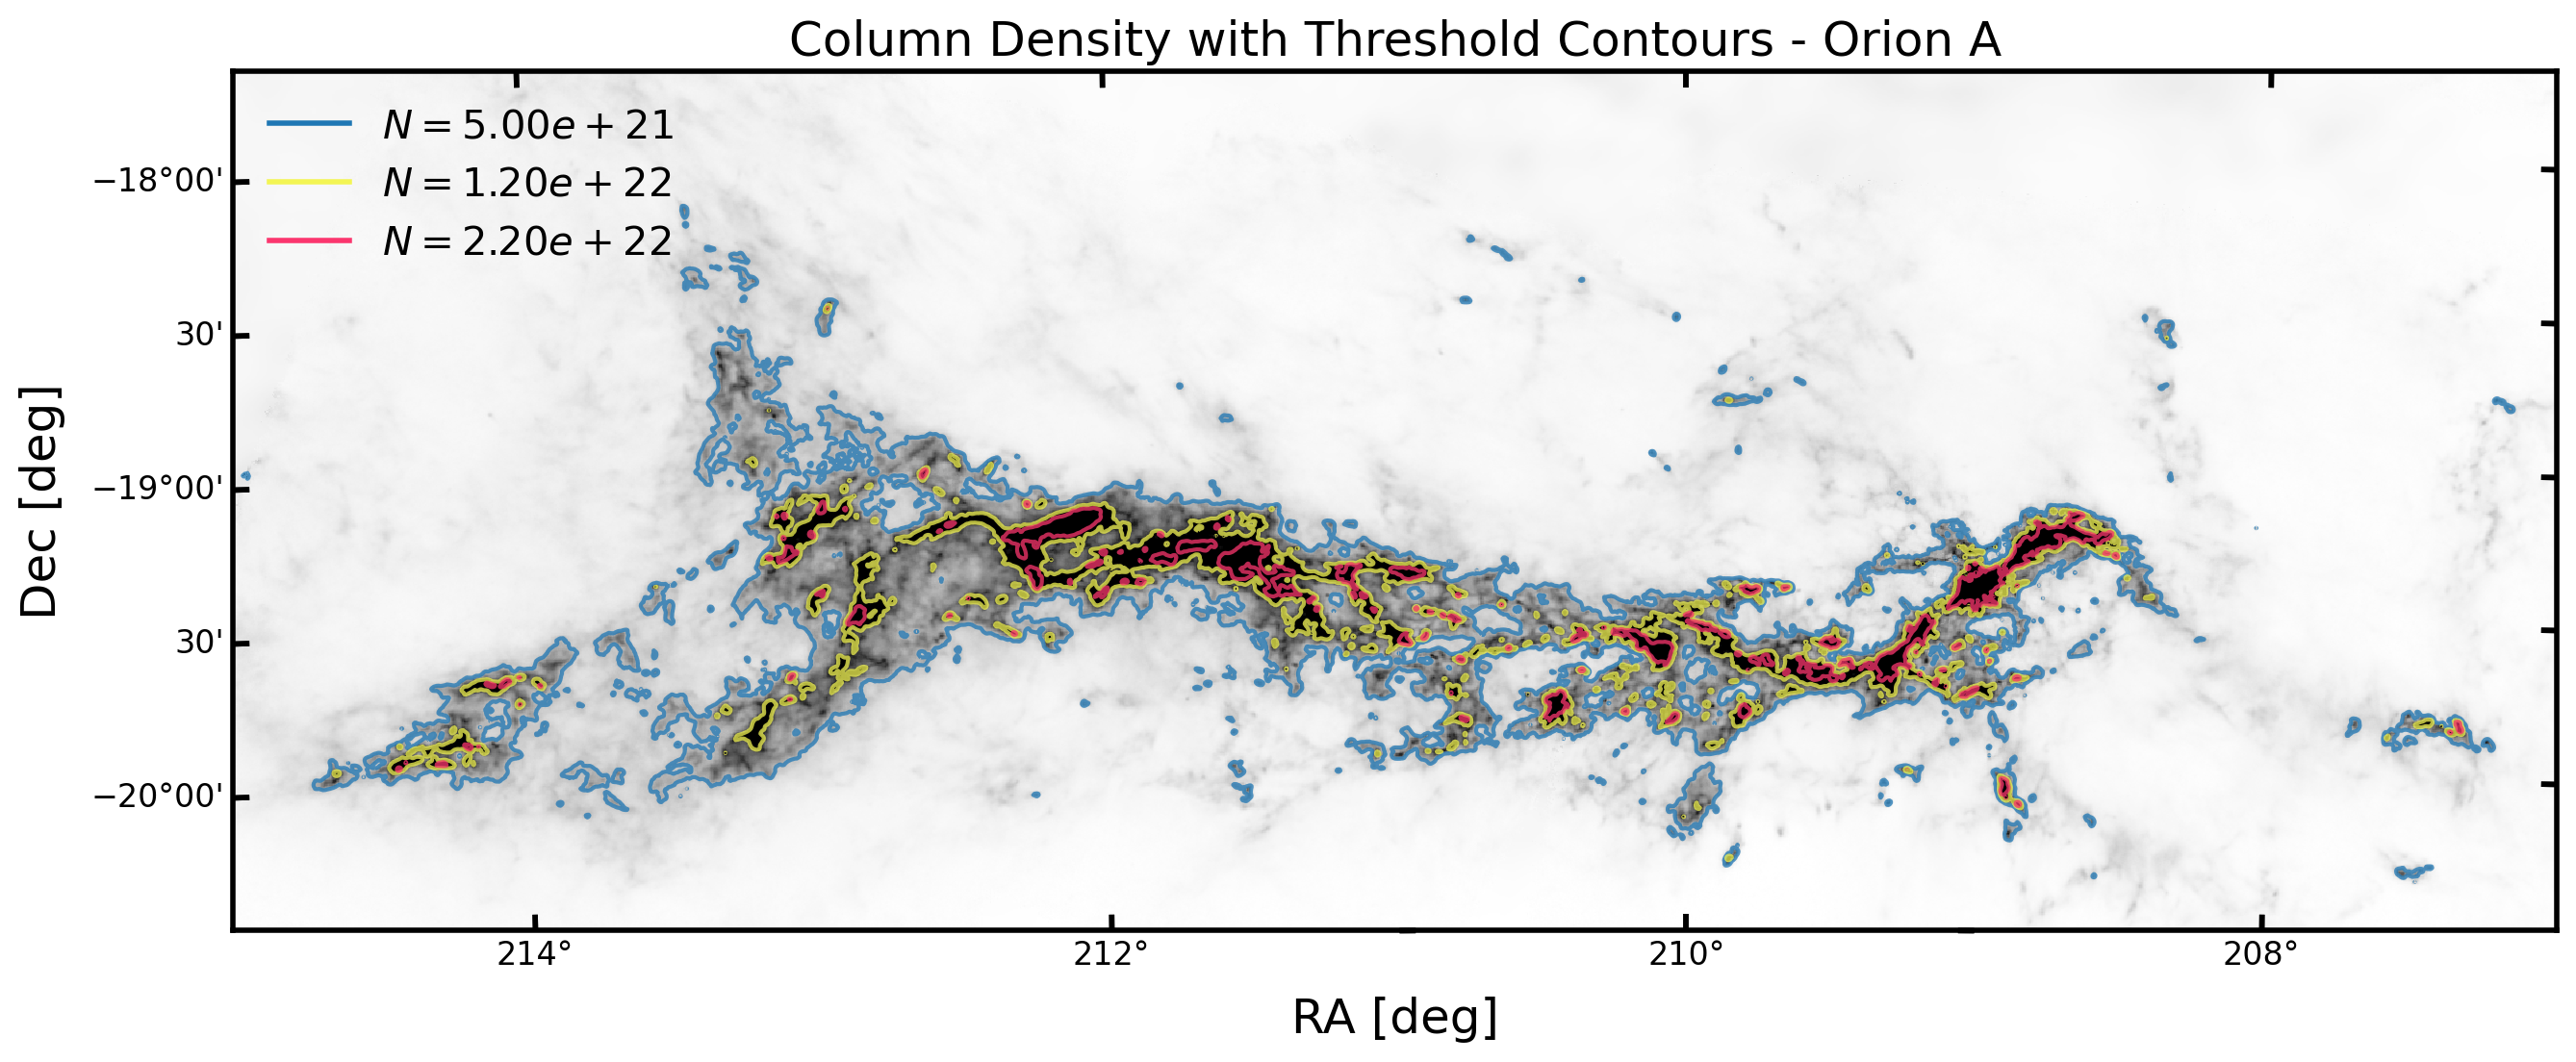
\includegraphics[width=0.83\textwidth]{figures/Orion_A_gallery_global.png}
    \caption{Column-density map of Orion~A with contours of three characteristic thresholds.}
    \label{fig:gallery_global_thresholds_OA}
\end{figure}

\begin{figure}[h]
    \centering
    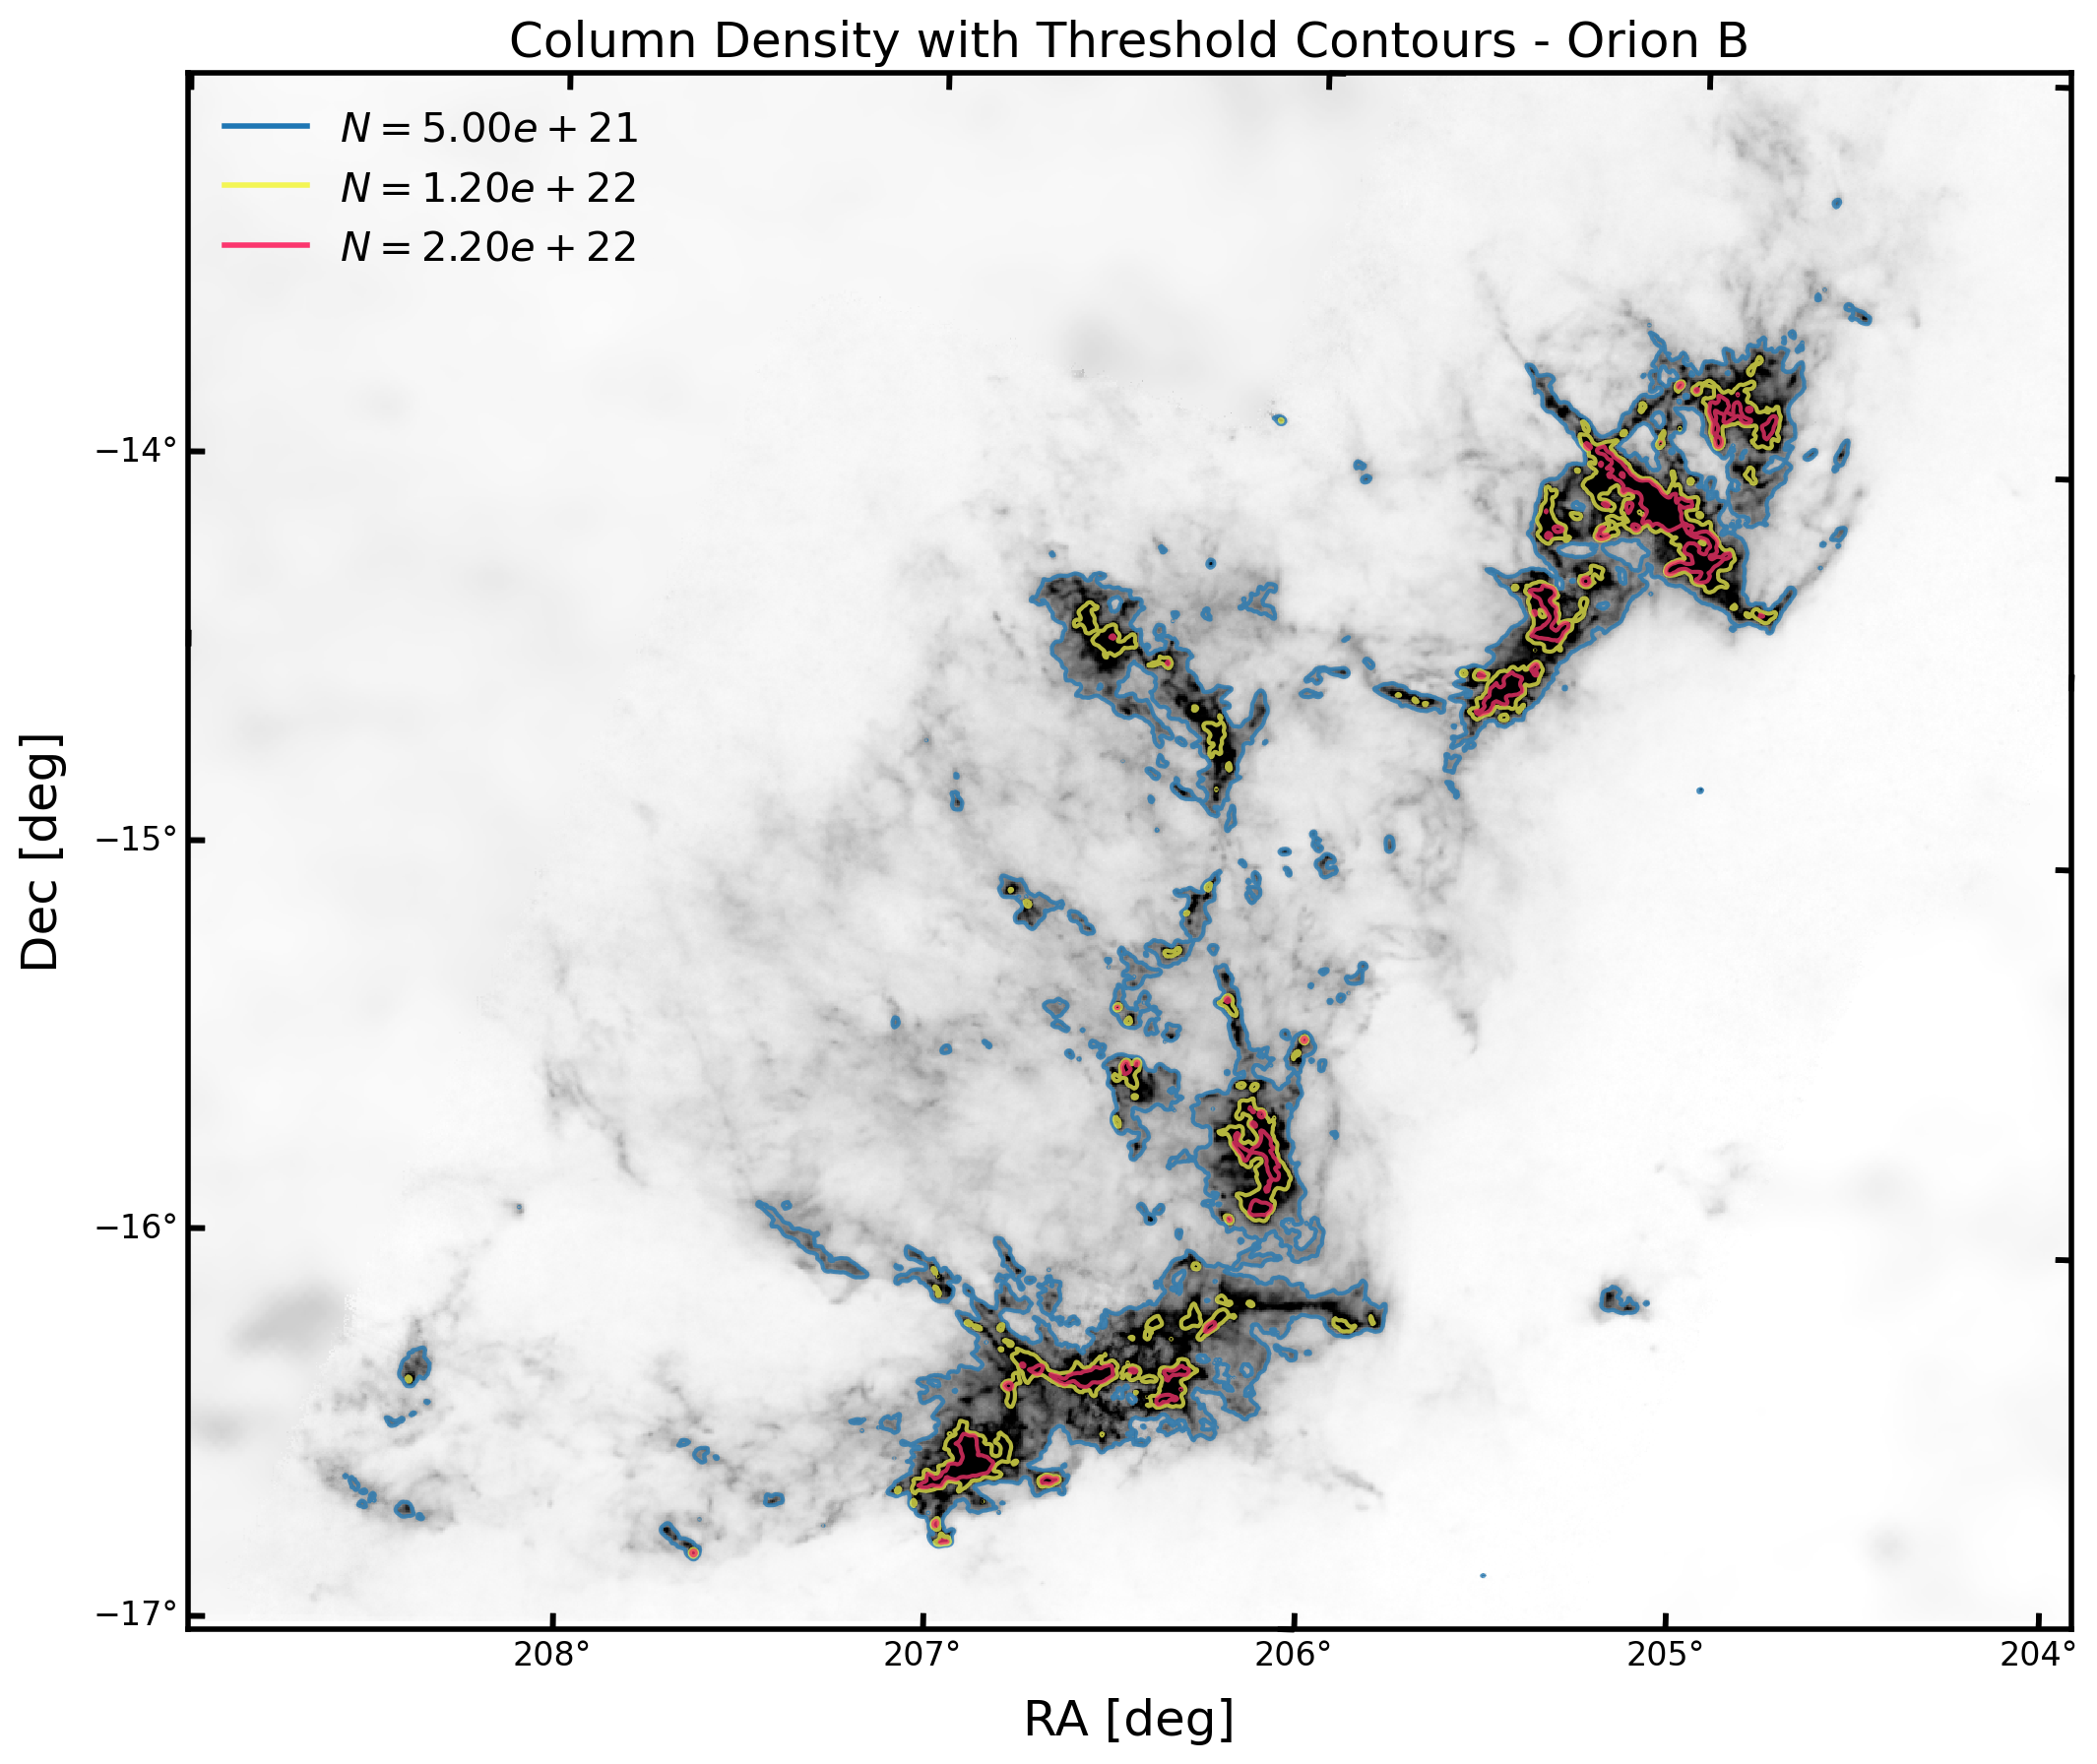
\includegraphics[width=0.64\textwidth]{figures/Orion_B_gallery_global.png}
    \caption{Column-density map of Orion~B with contours as in Figure~\ref{fig:gallery_global_thresholds_OA}.}
    \label{fig:gallery_global_thresholds_OB}
\end{figure}

\section{Euler Characteristic}

\begin{figure}[h]
    \centering
    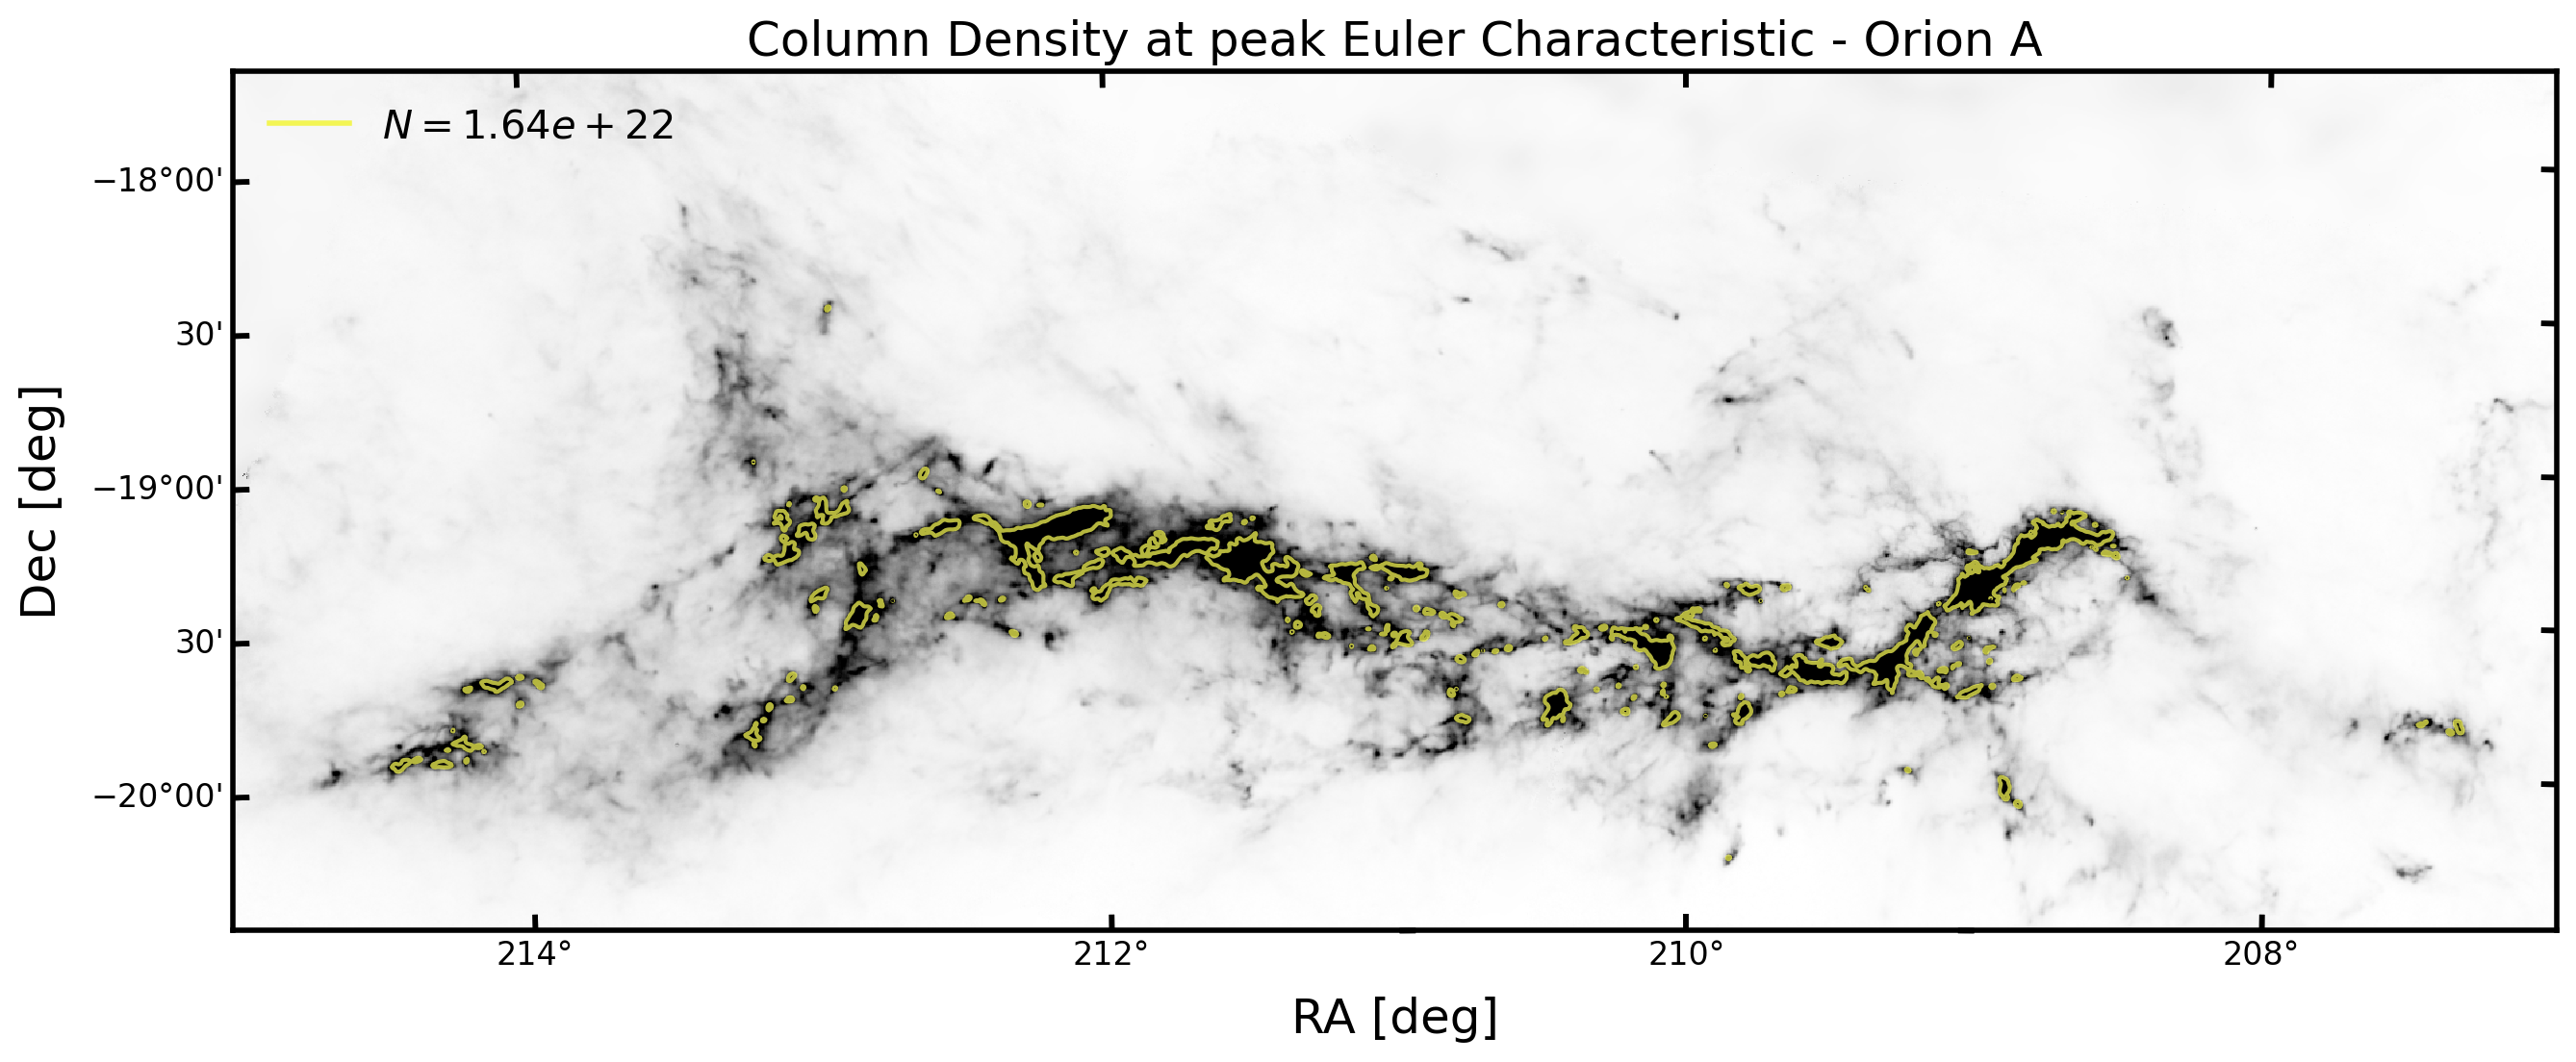
\includegraphics[width=0.79\textwidth]{figures/Euler_Orion_A_gallery.png}
    \caption{Column-density map of Orion~A with a contour overlaid at the threshold corresponding to the peak in the Euler characteristic.}
    \label{fig:gallery_euler_OA}
\end{figure}

\begin{figure}[h]
    \centering
    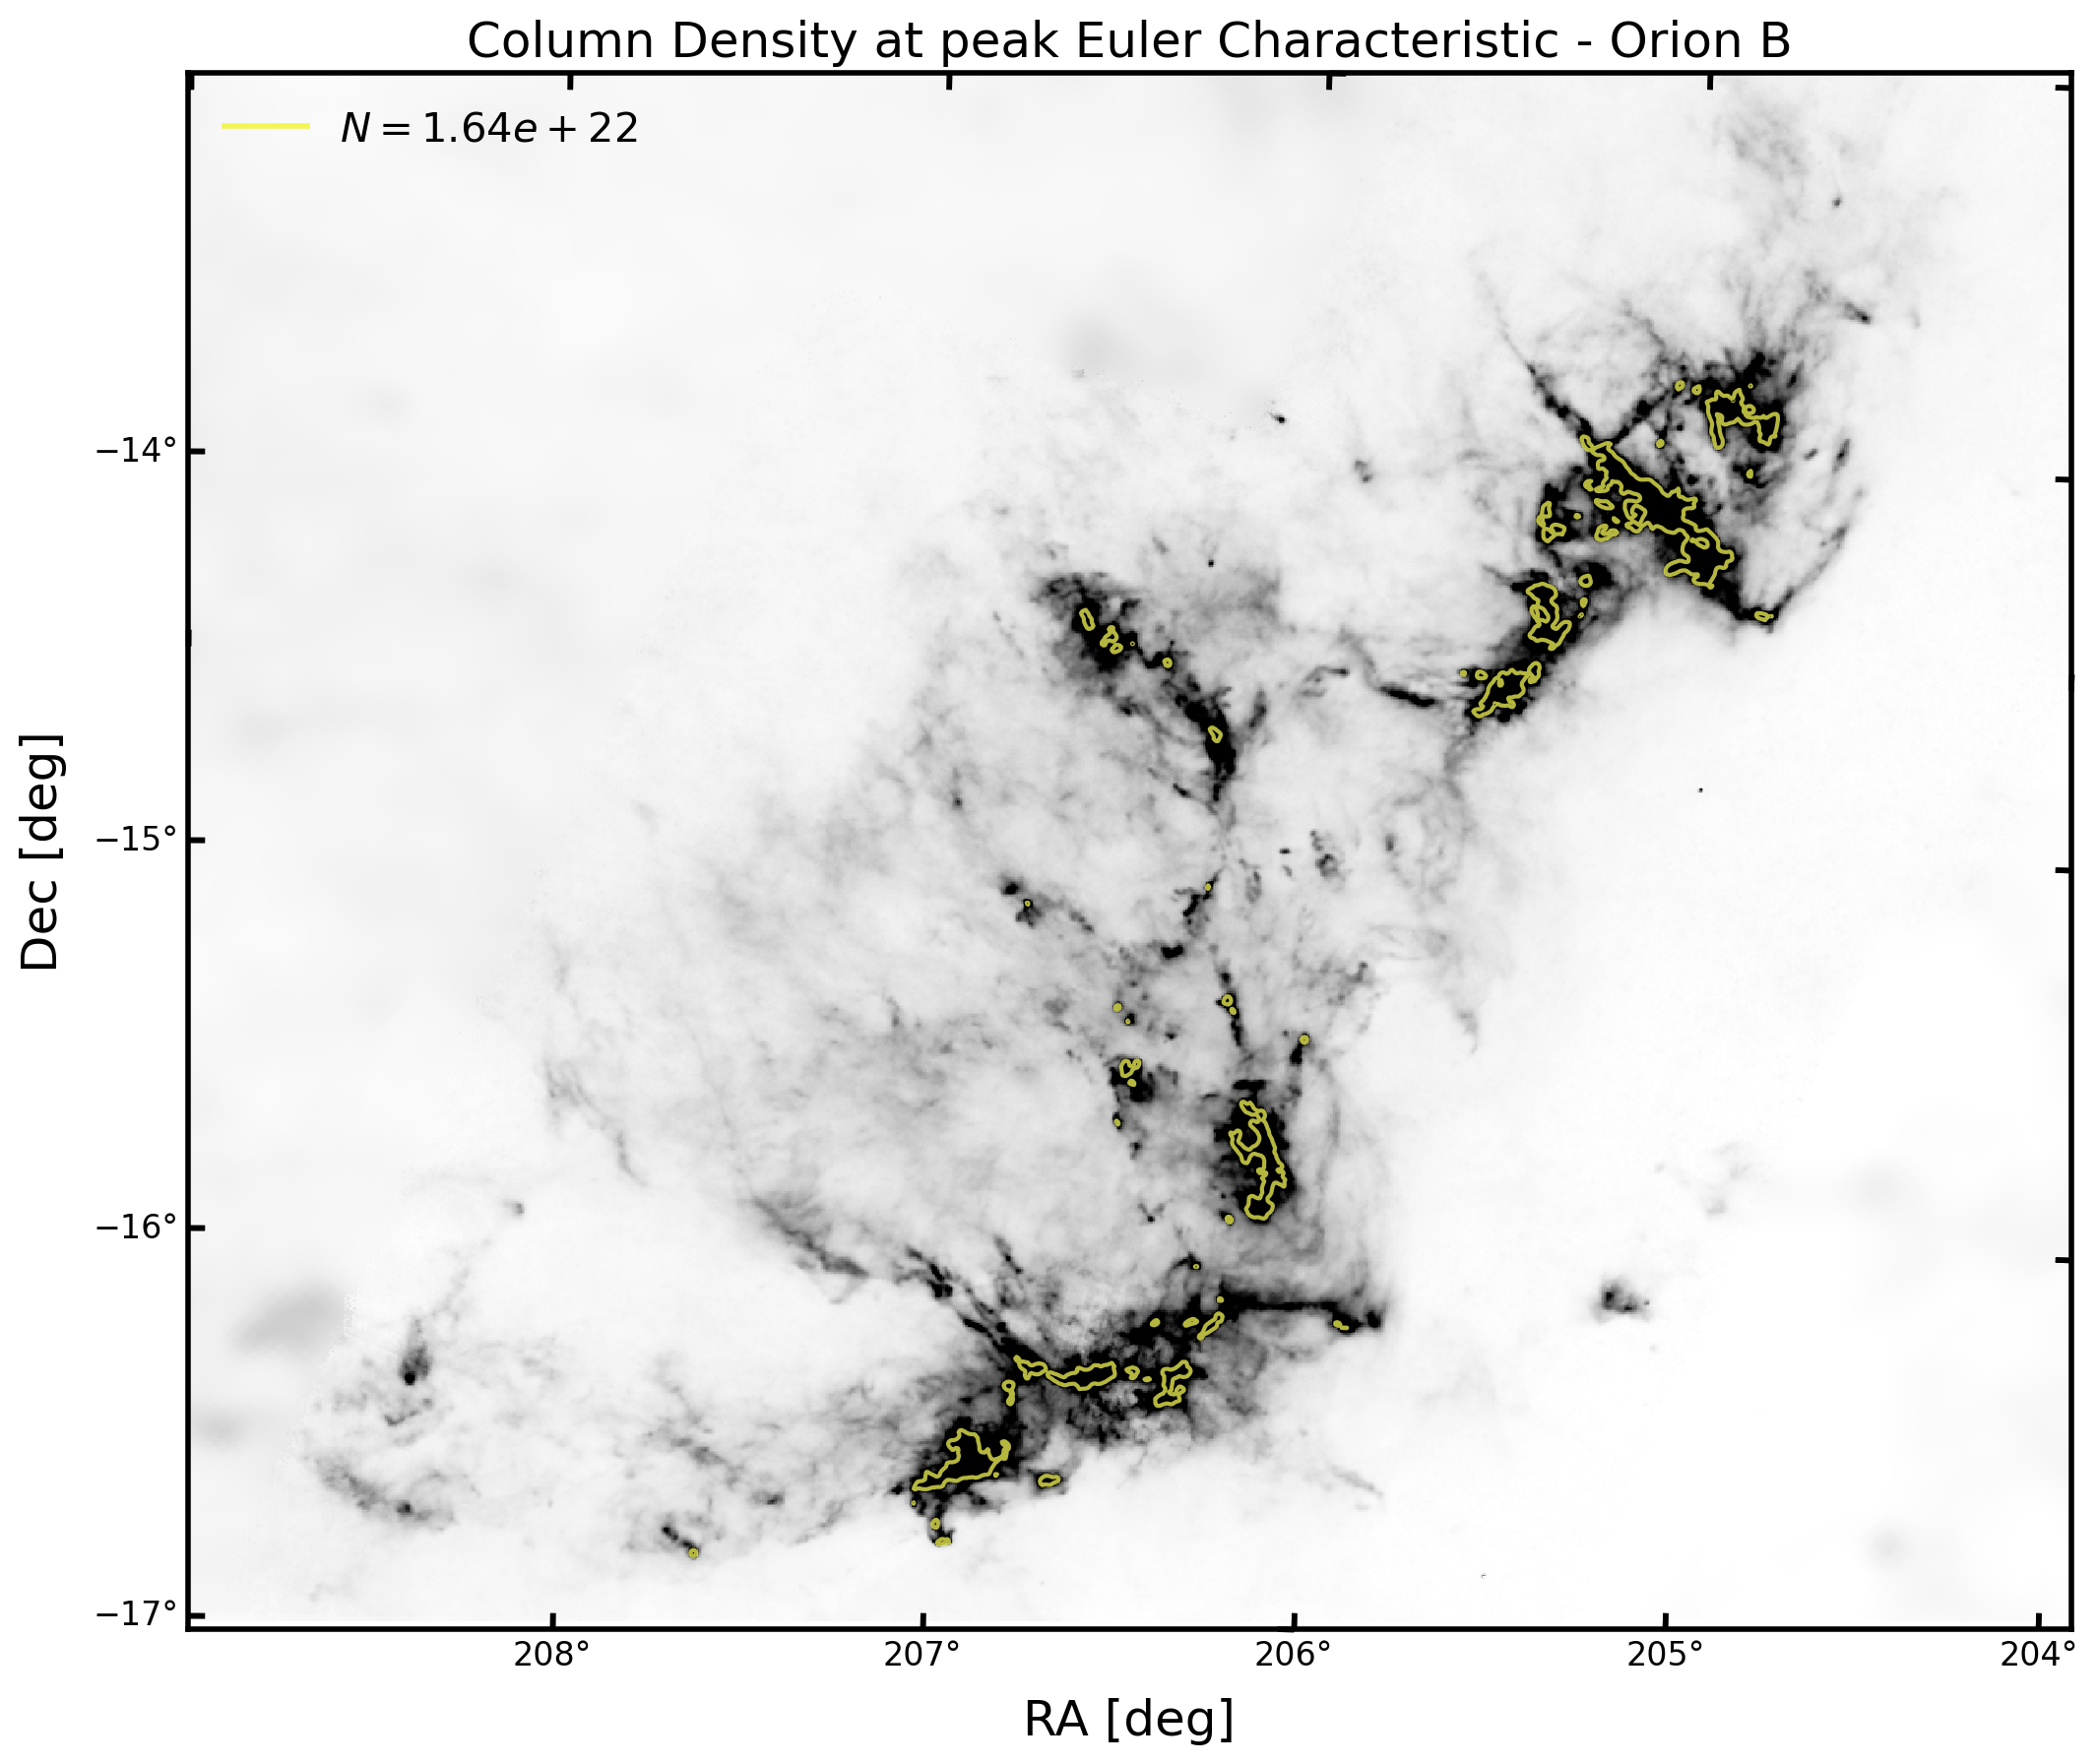
\includegraphics[width=0.57\textwidth]{figures/Euler_Orion_B_gallery.png}
    \caption{Column-density map of Orion~B with a contour overlaid at the same threshold used for Orion~A in Figure~\ref{fig:gallery_euler_OA}. While this value does not correspond to a peak in Orion~B’s Euler characteristic, it is shown here for visual comparison.}
    \label{fig:gallery_euler_OB}
\end{figure}

\clearpage

\section{Local Fractal Dimension}
% confirmation of increasing network of overall complexity
% peaks 

\clearpage

\section{MSD}

\begin{figure}[h]
    \centering
    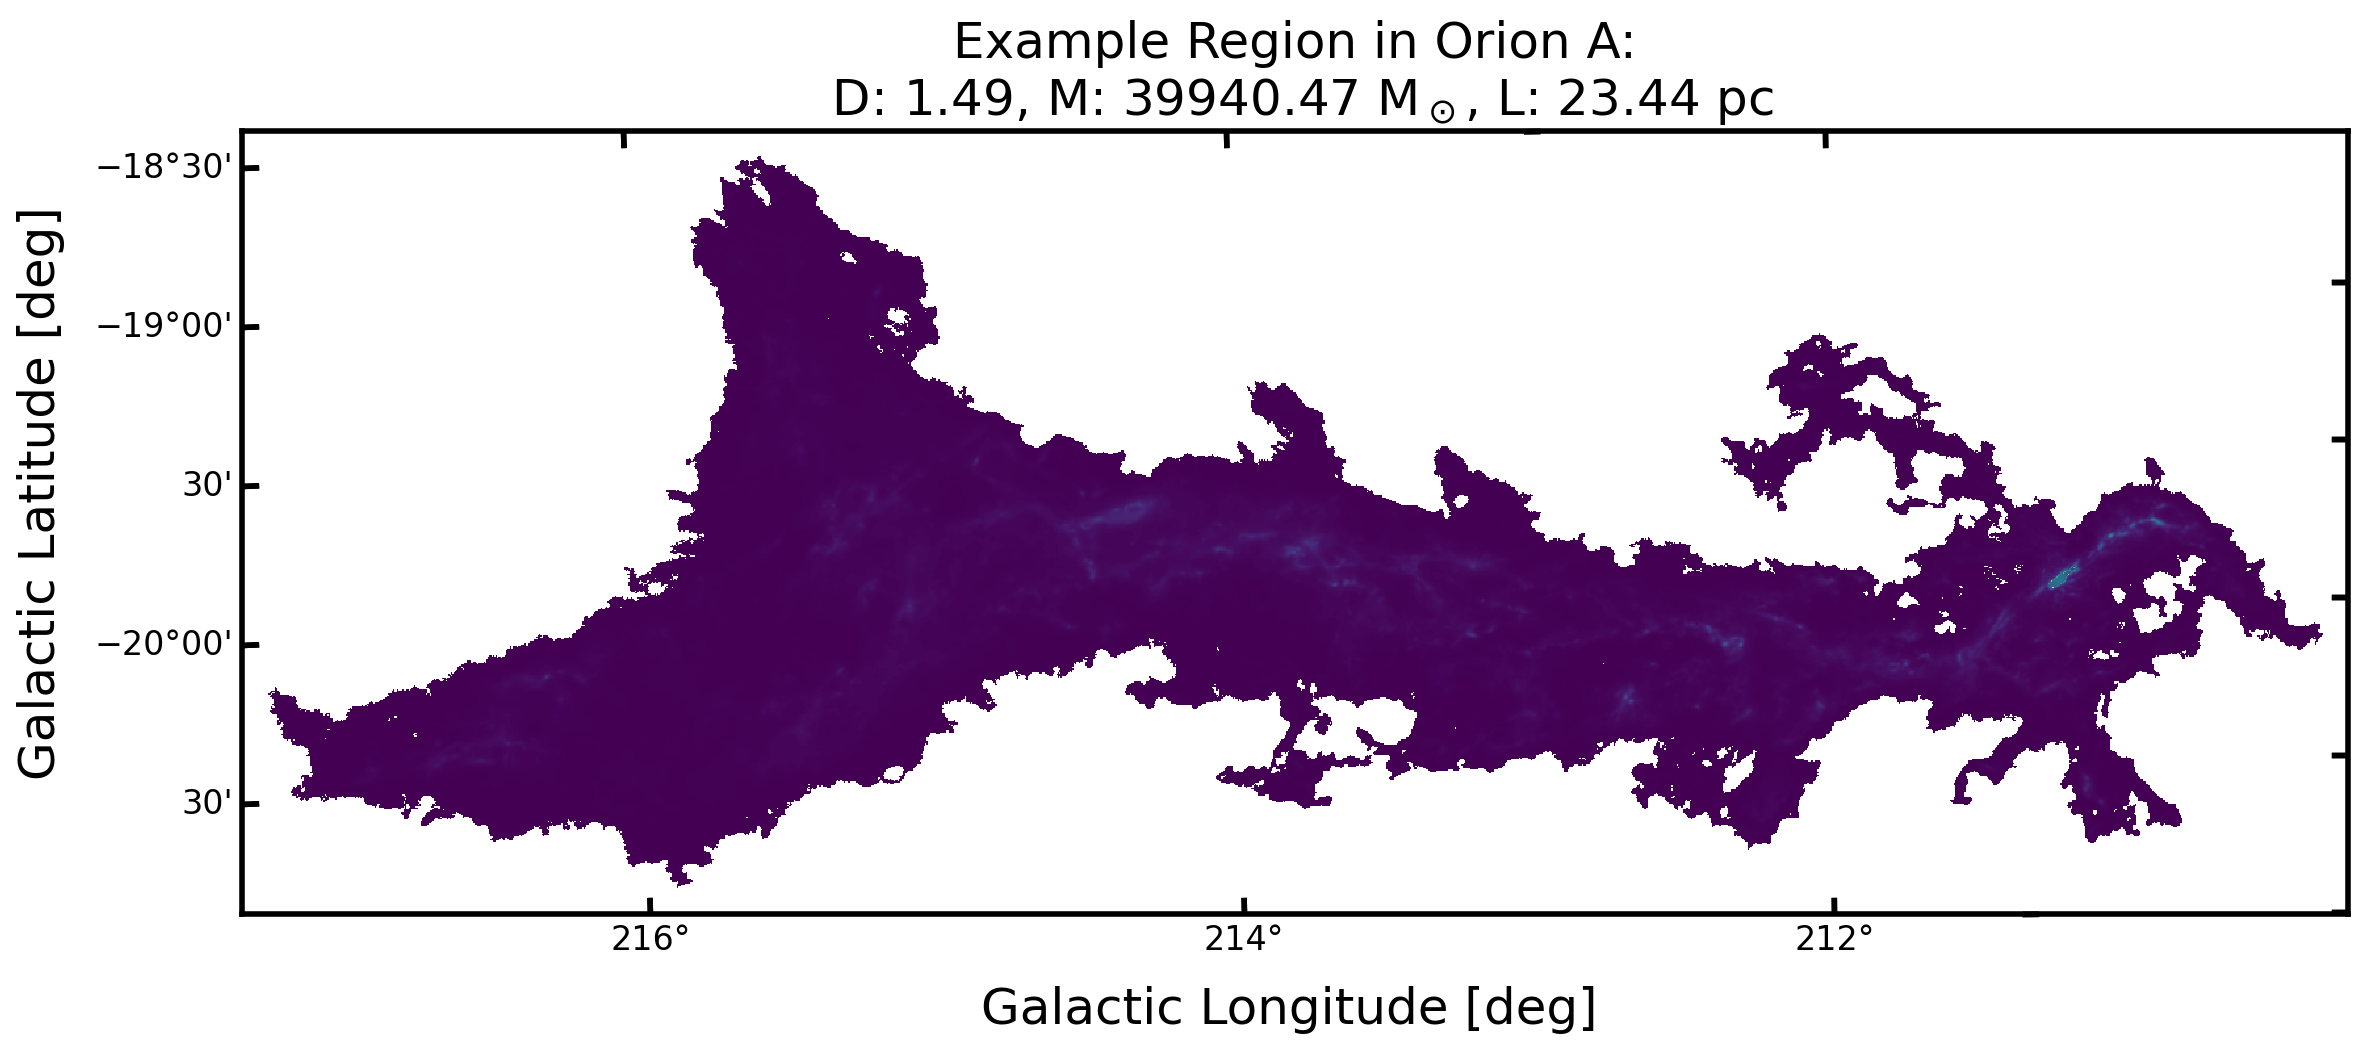
\includegraphics[width=0.84\textwidth]{figures/MSD_Gallery_Orion_A_1.png}
    \caption{Example of the mask of an individual structure extracted from Orion~A at a given column density threshold. Key physical properties—mass, size, and local fractal dimension—are indicated in the title of the plot.}
    \label{fig:gallery_MSD_A_1}
\end{figure}

\begin{figure}[h]
    \centering
    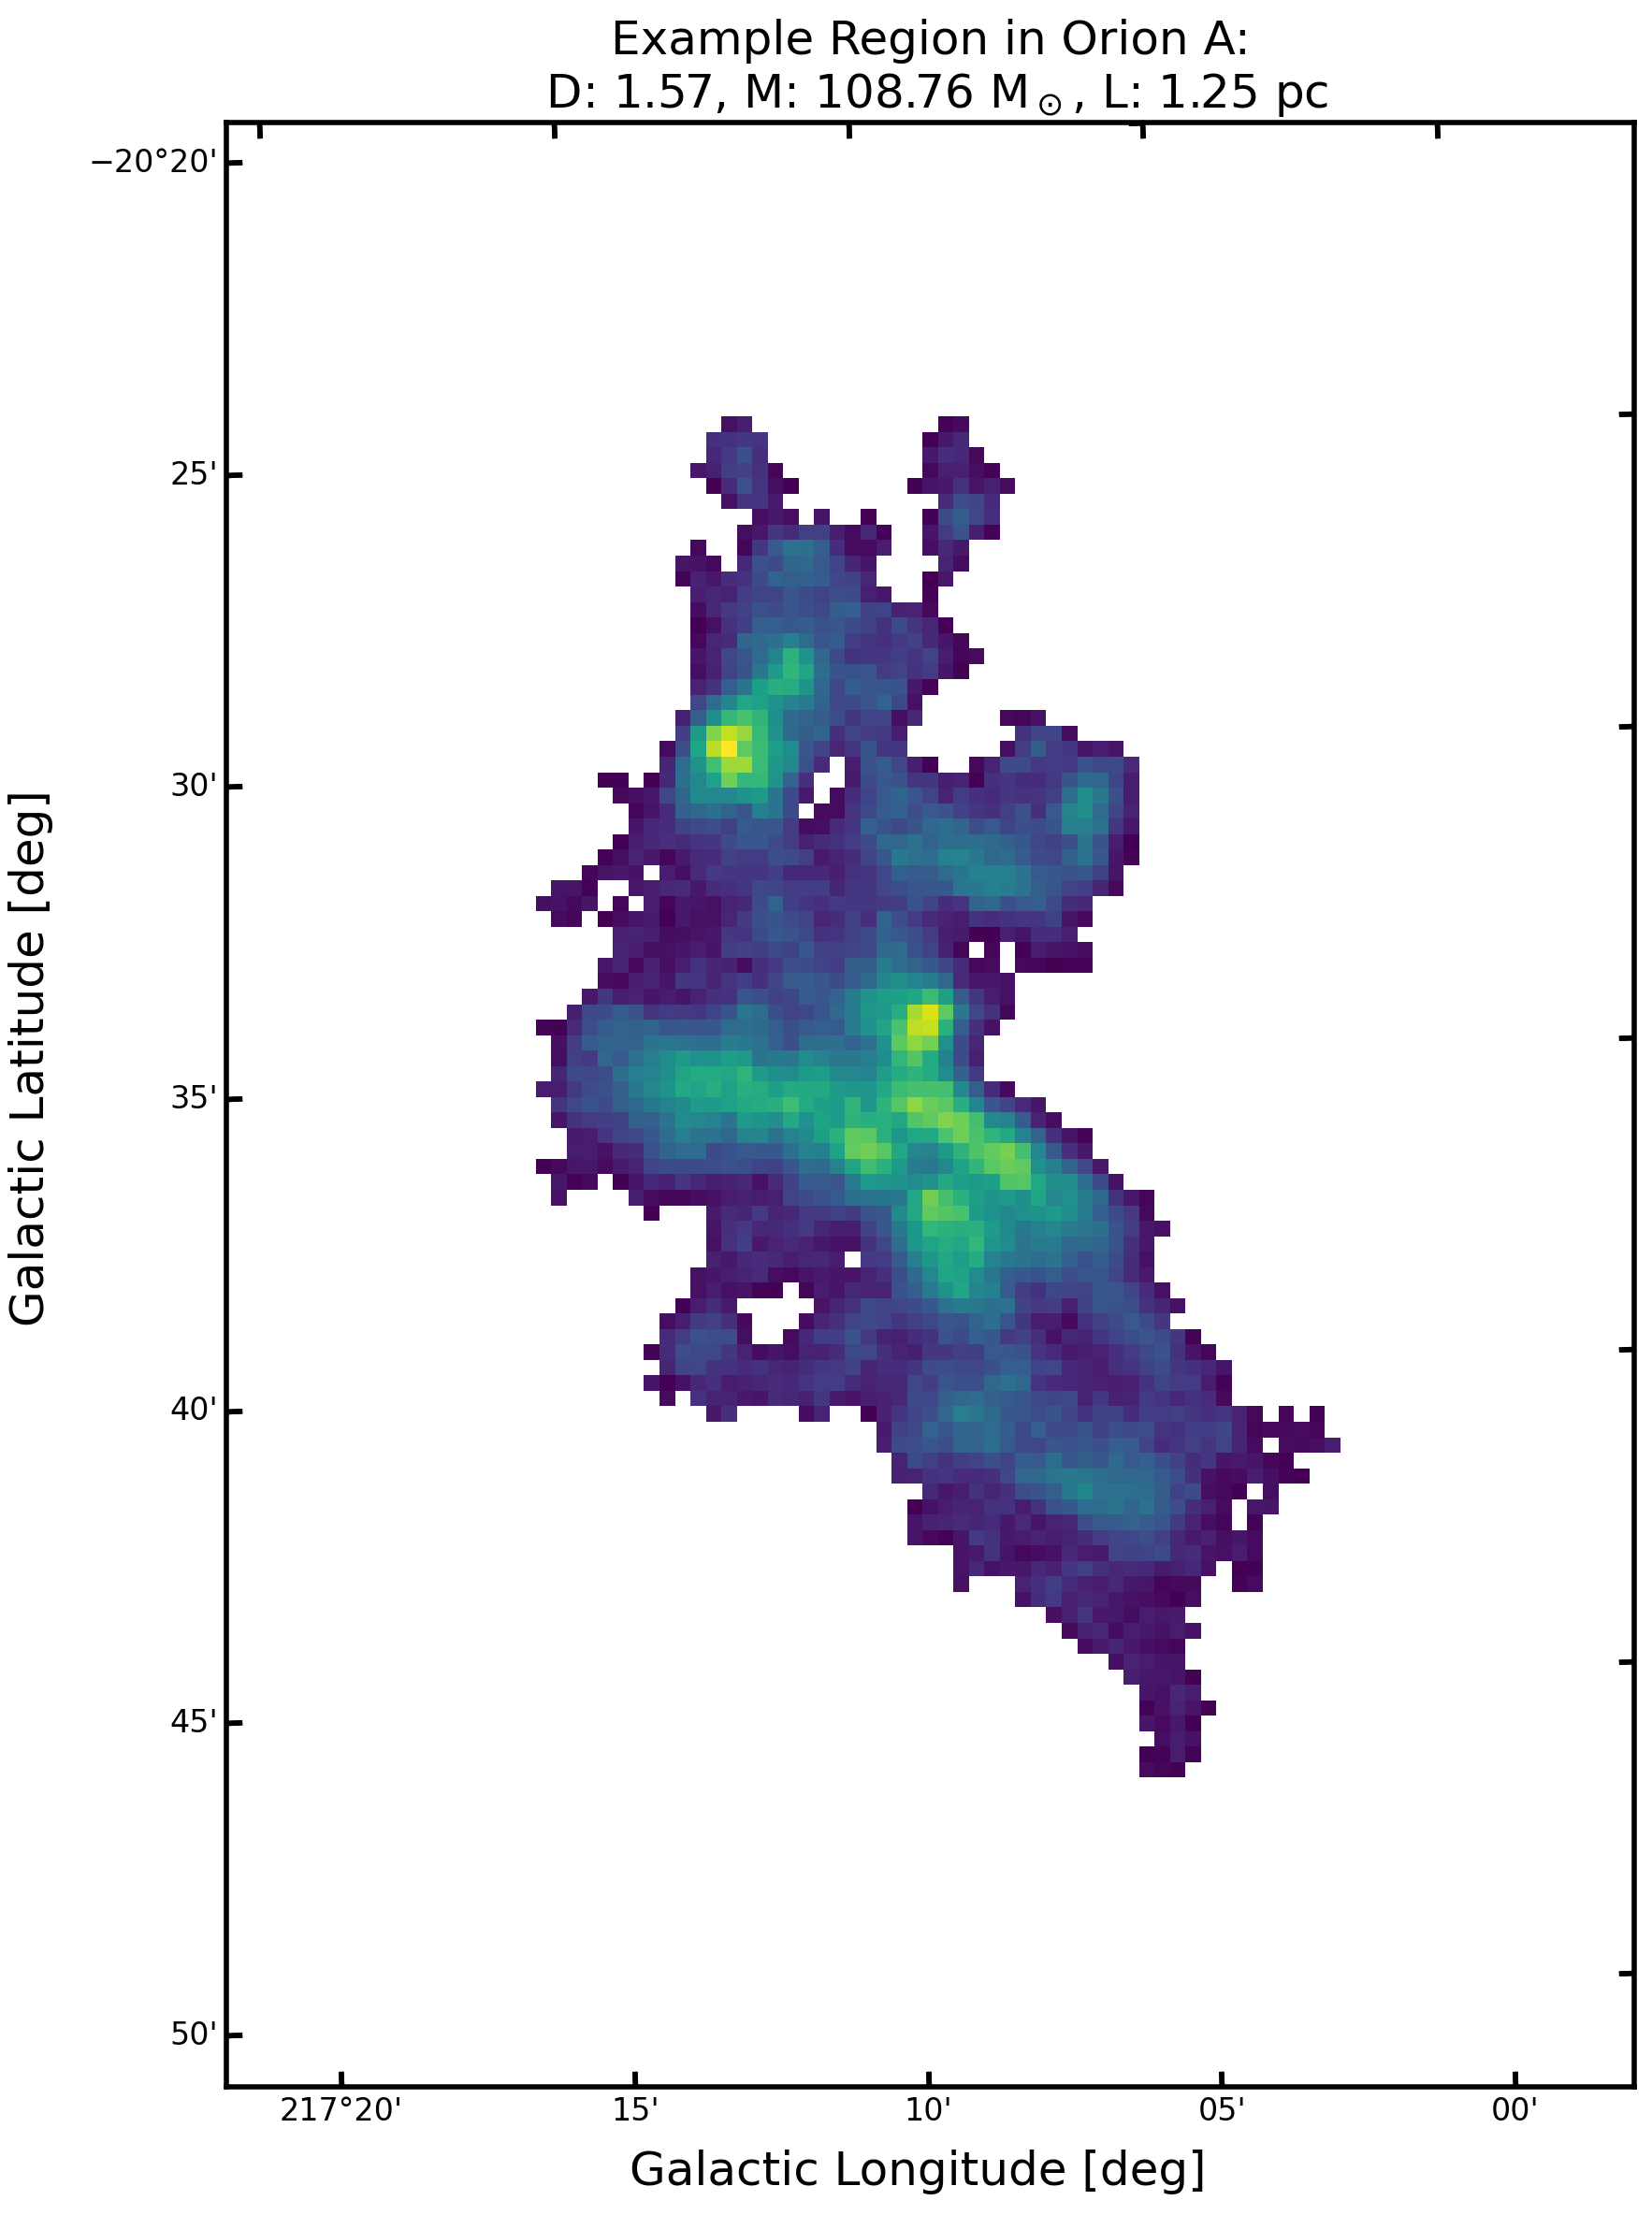
\includegraphics[width=0.6\textwidth]{figures/MSD_Gallery_Orion_A_2.png}
    \caption{Example of the mask of an individual structure extracted from Orion~A at a given column density threshold.}
    \label{fig:gallery_MSD_A_2}
\end{figure}

\begin{figure}[h]
    \centering
    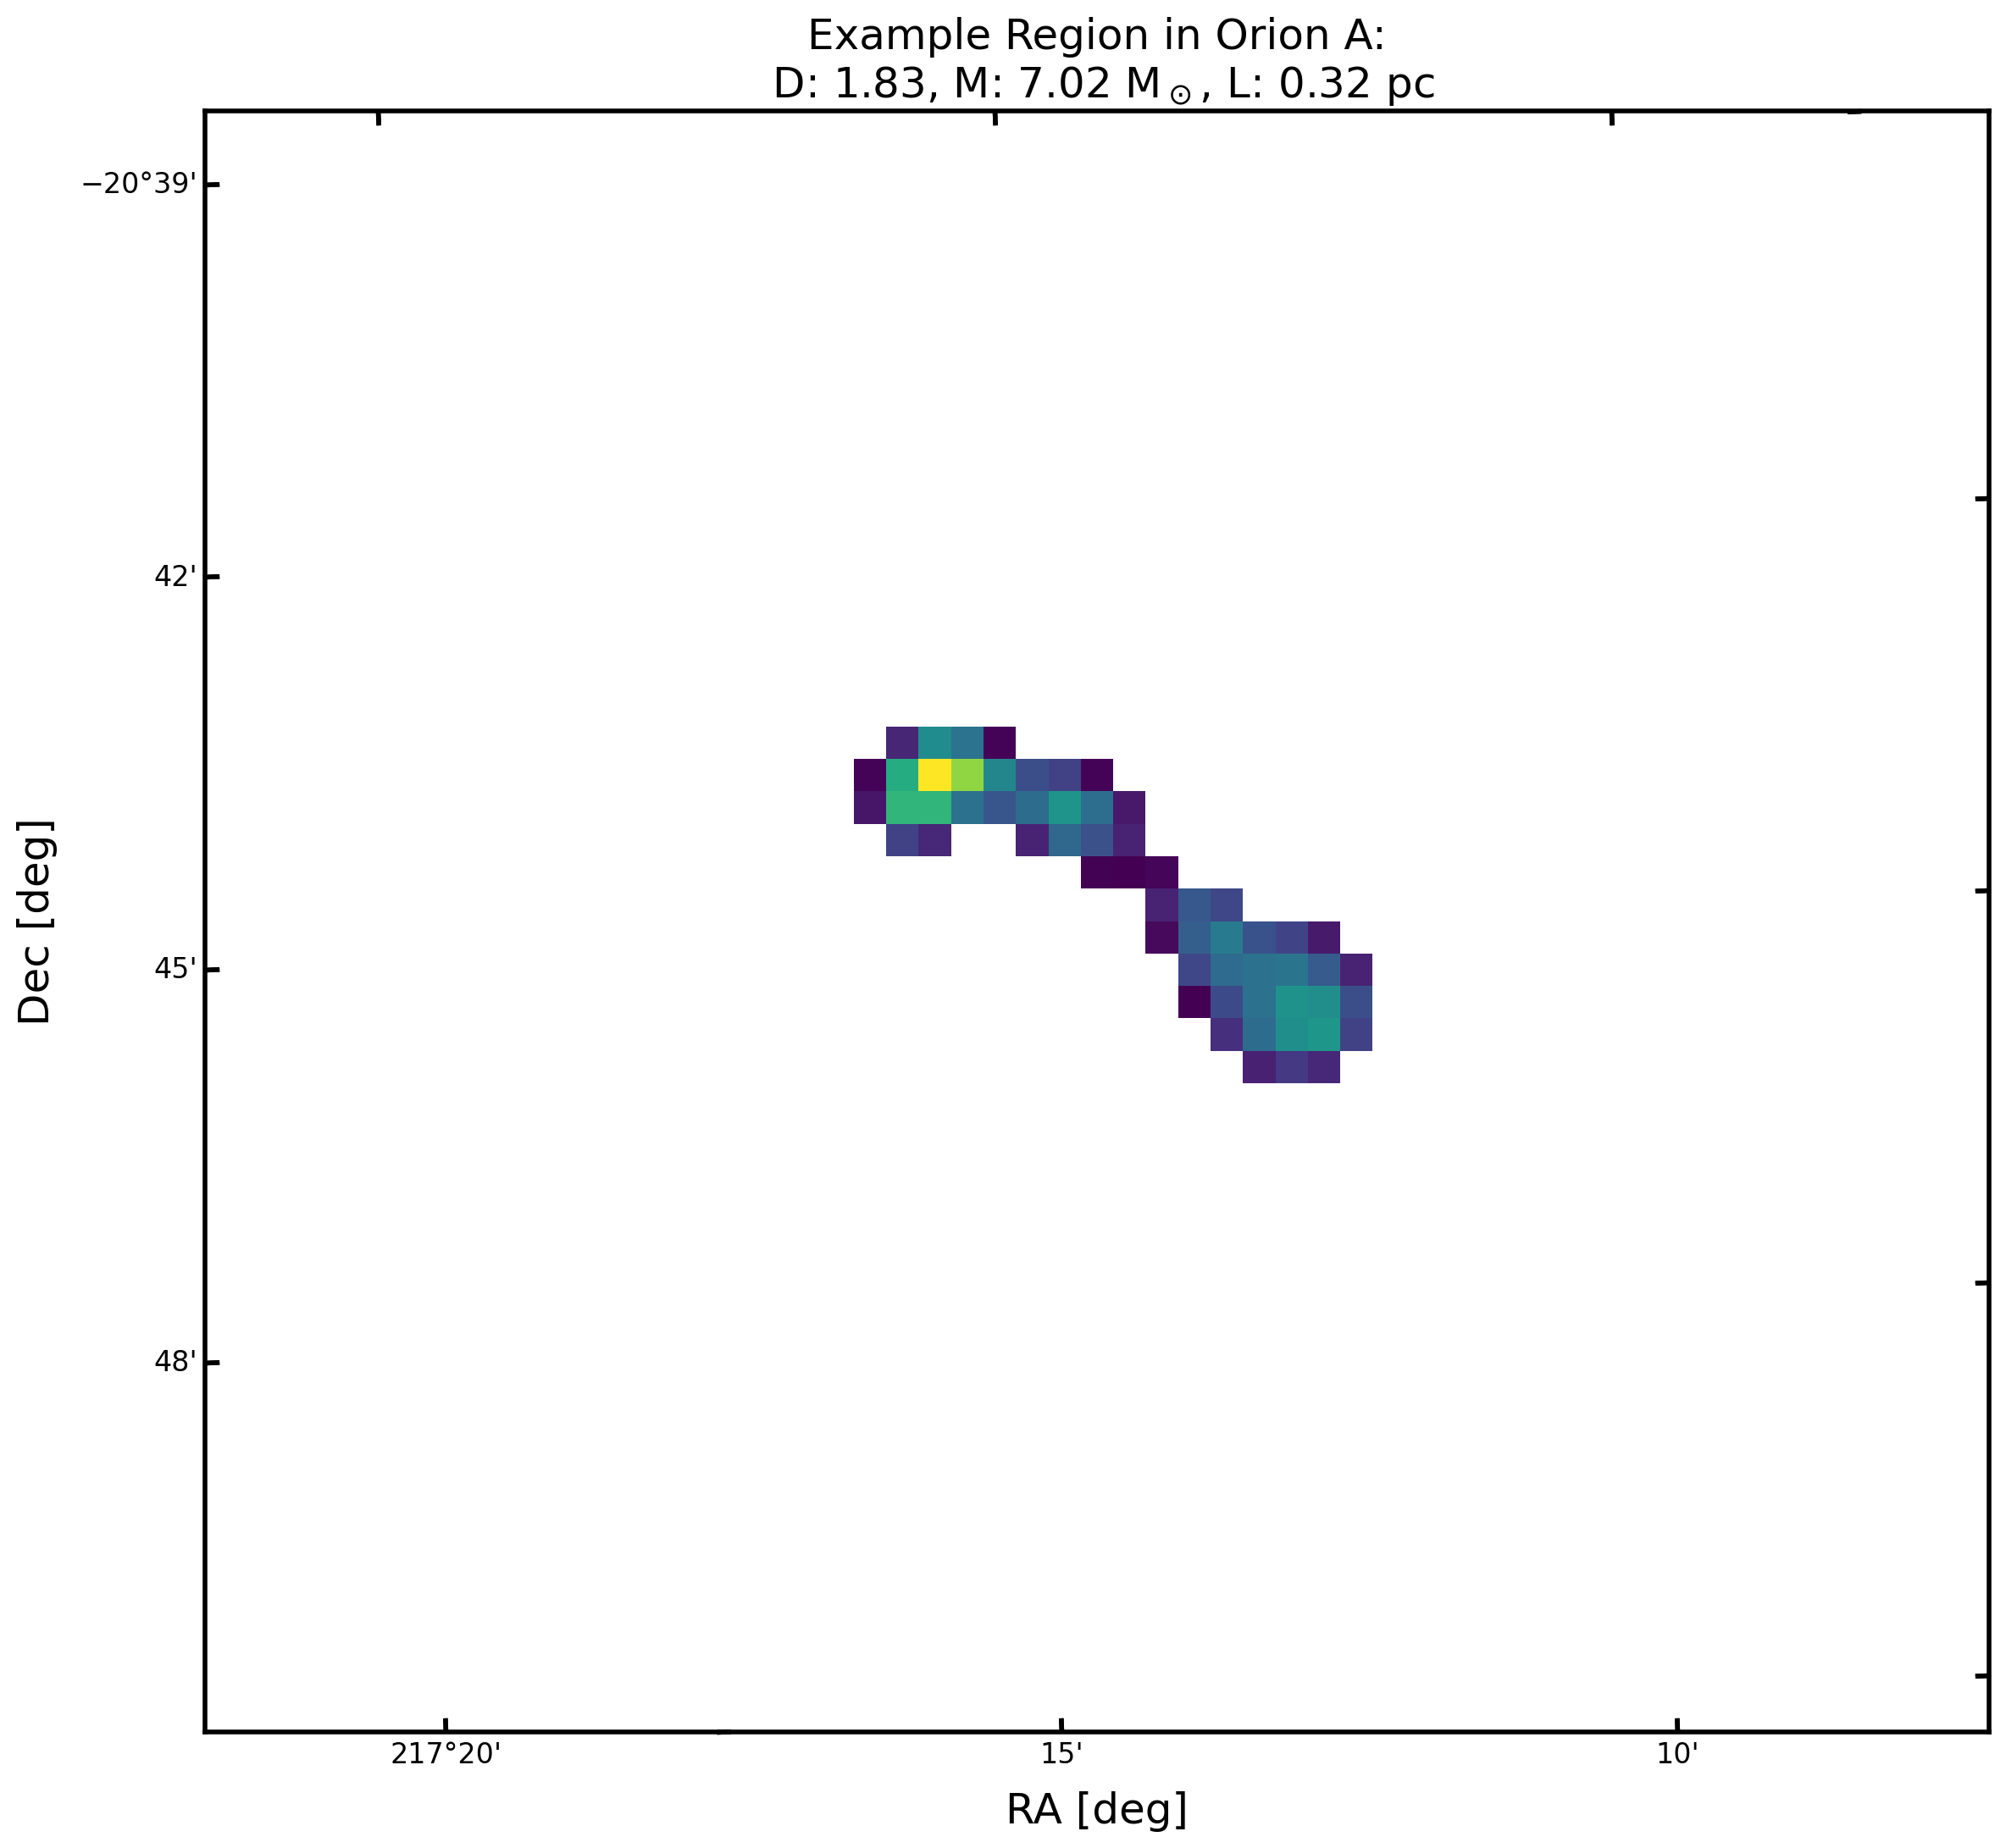
\includegraphics[width=0.6\textwidth]{figures/MSD_Gallery_Orion_A_3.png}
    \caption{Example of the mask of an individual structure extracted from Orion~A at a given column density threshold.}
    \label{fig:gallery_MSD_A_3}
\end{figure}

\begin{figure}[h]
    \centering
    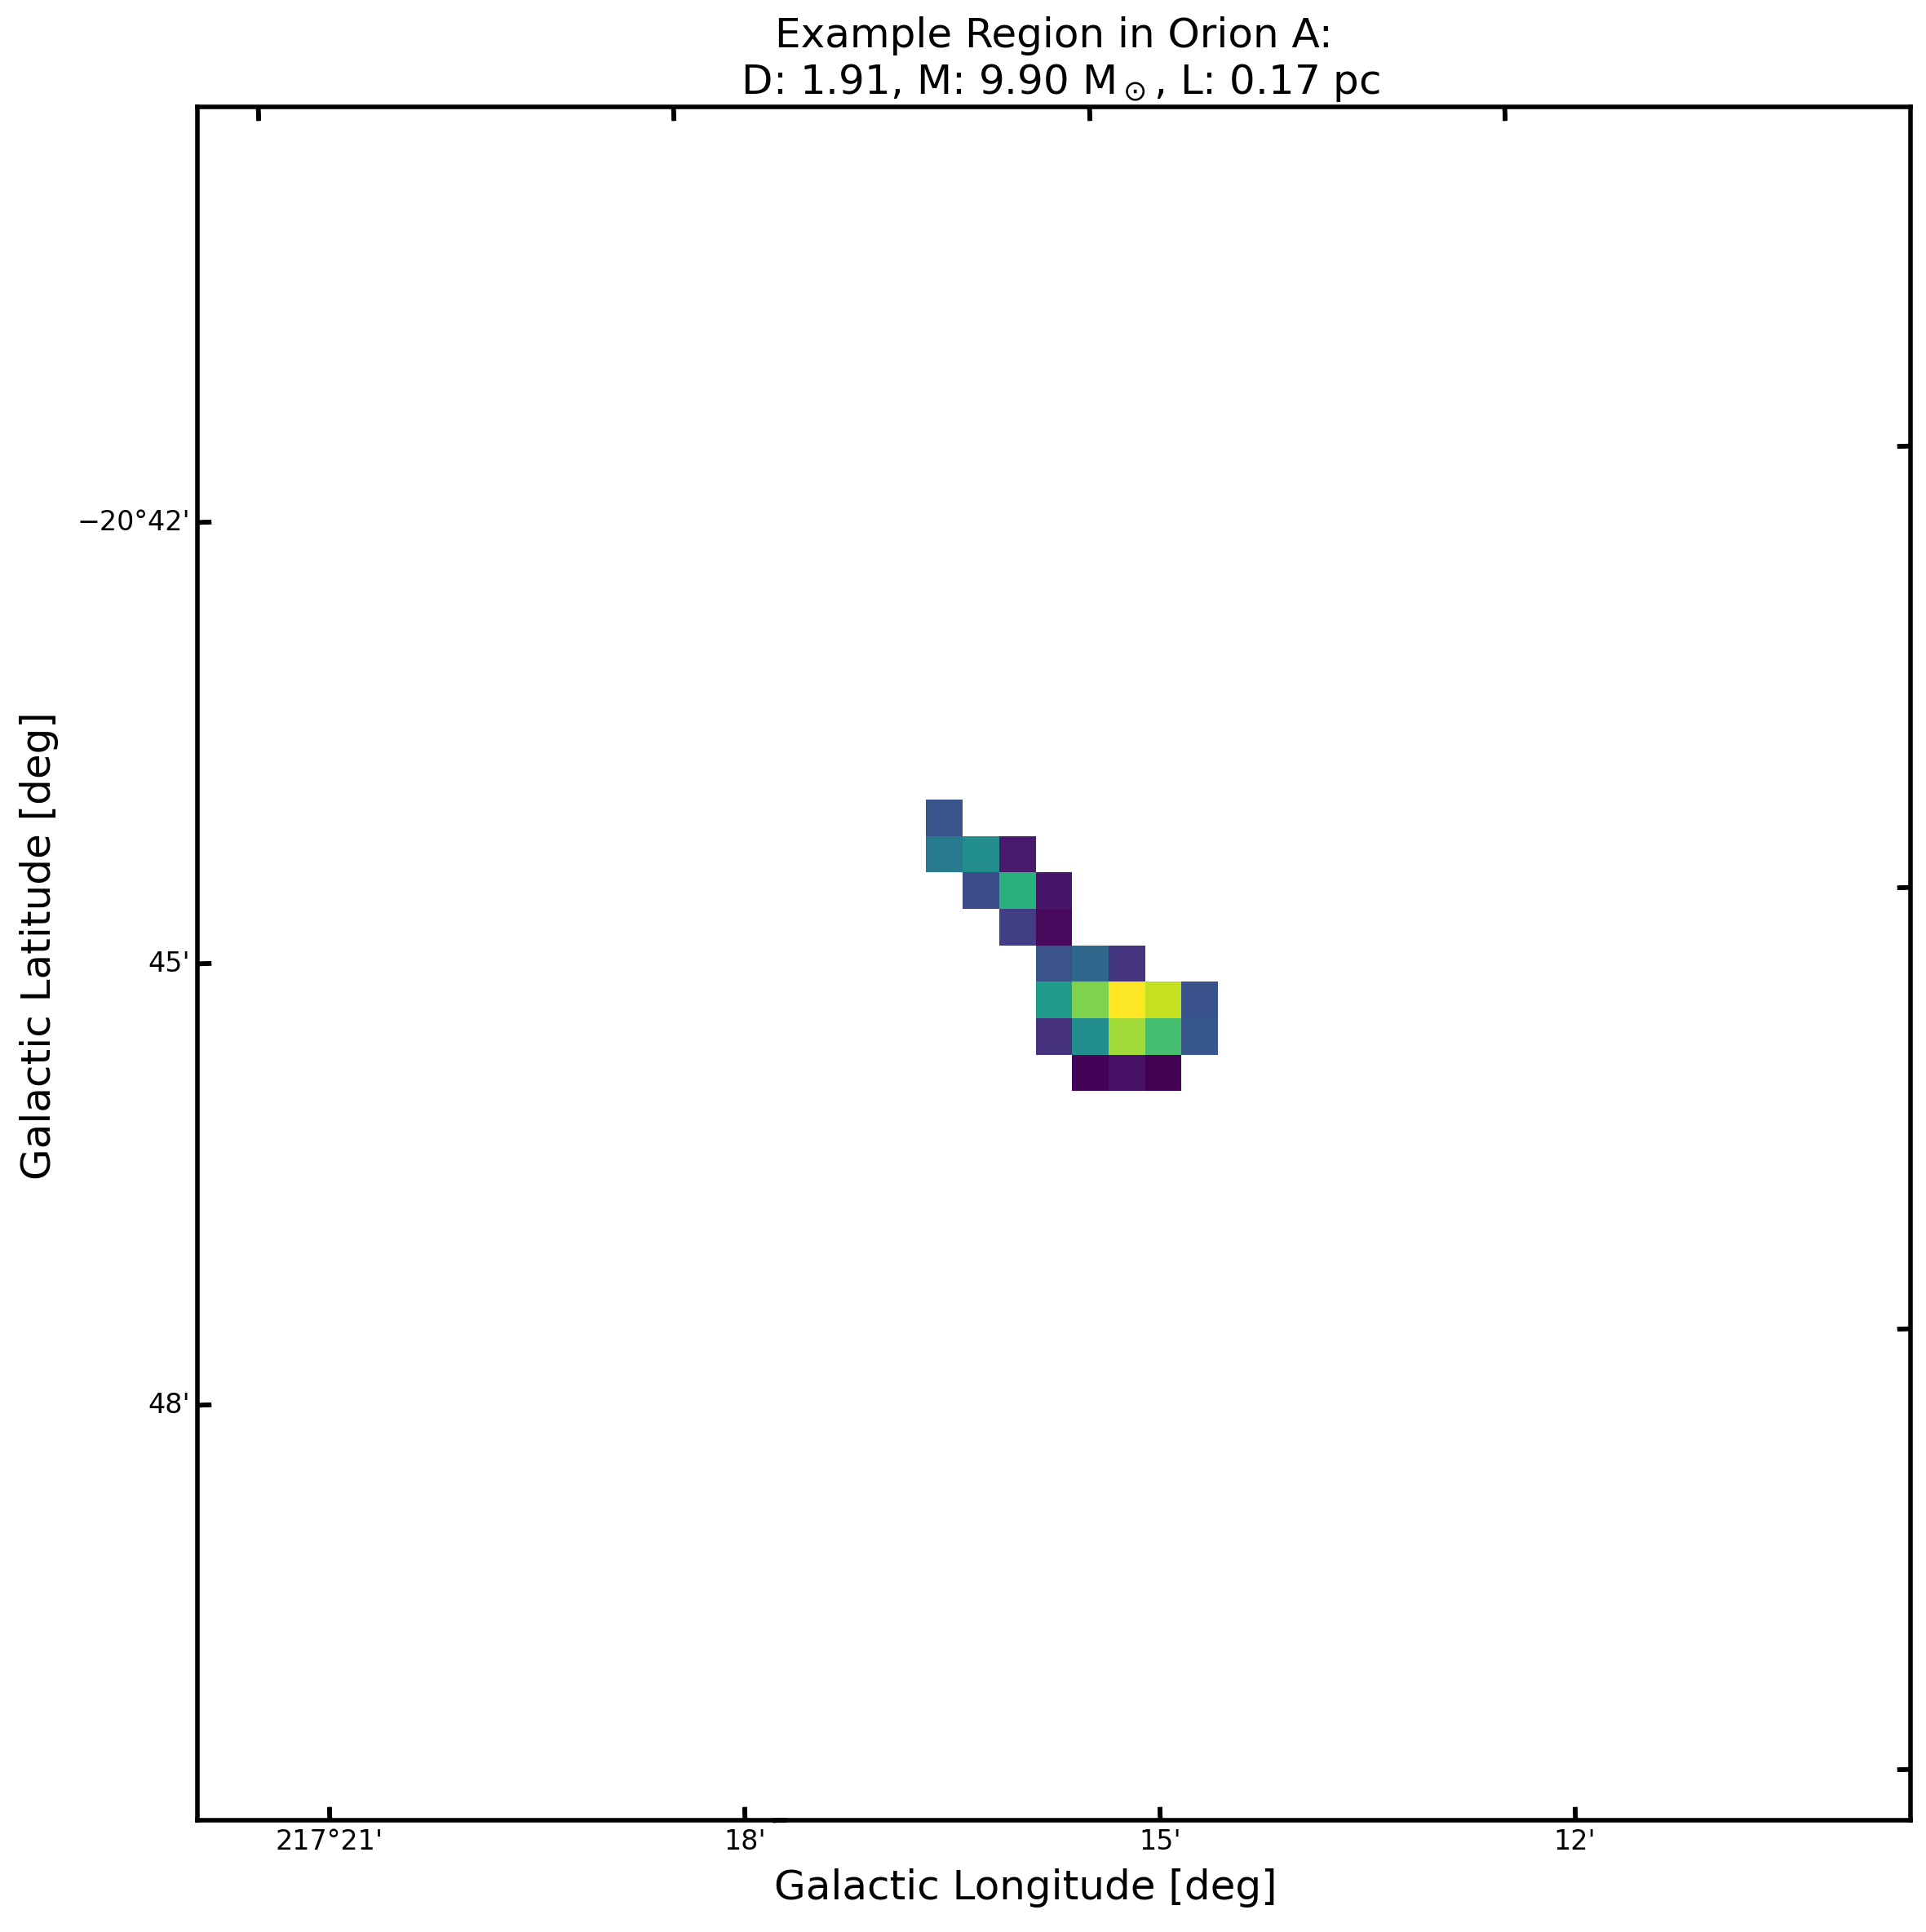
\includegraphics[width=0.6\textwidth]{figures/MSD_Gallery_Orion_A_4.png}
    \caption{Example of the mask of an individual structure extracted from Orion~A at a given column density threshold.}
    \label{fig:gallery_MSD_A_4}
\end{figure}

\begin{figure}[h]
    \centering
    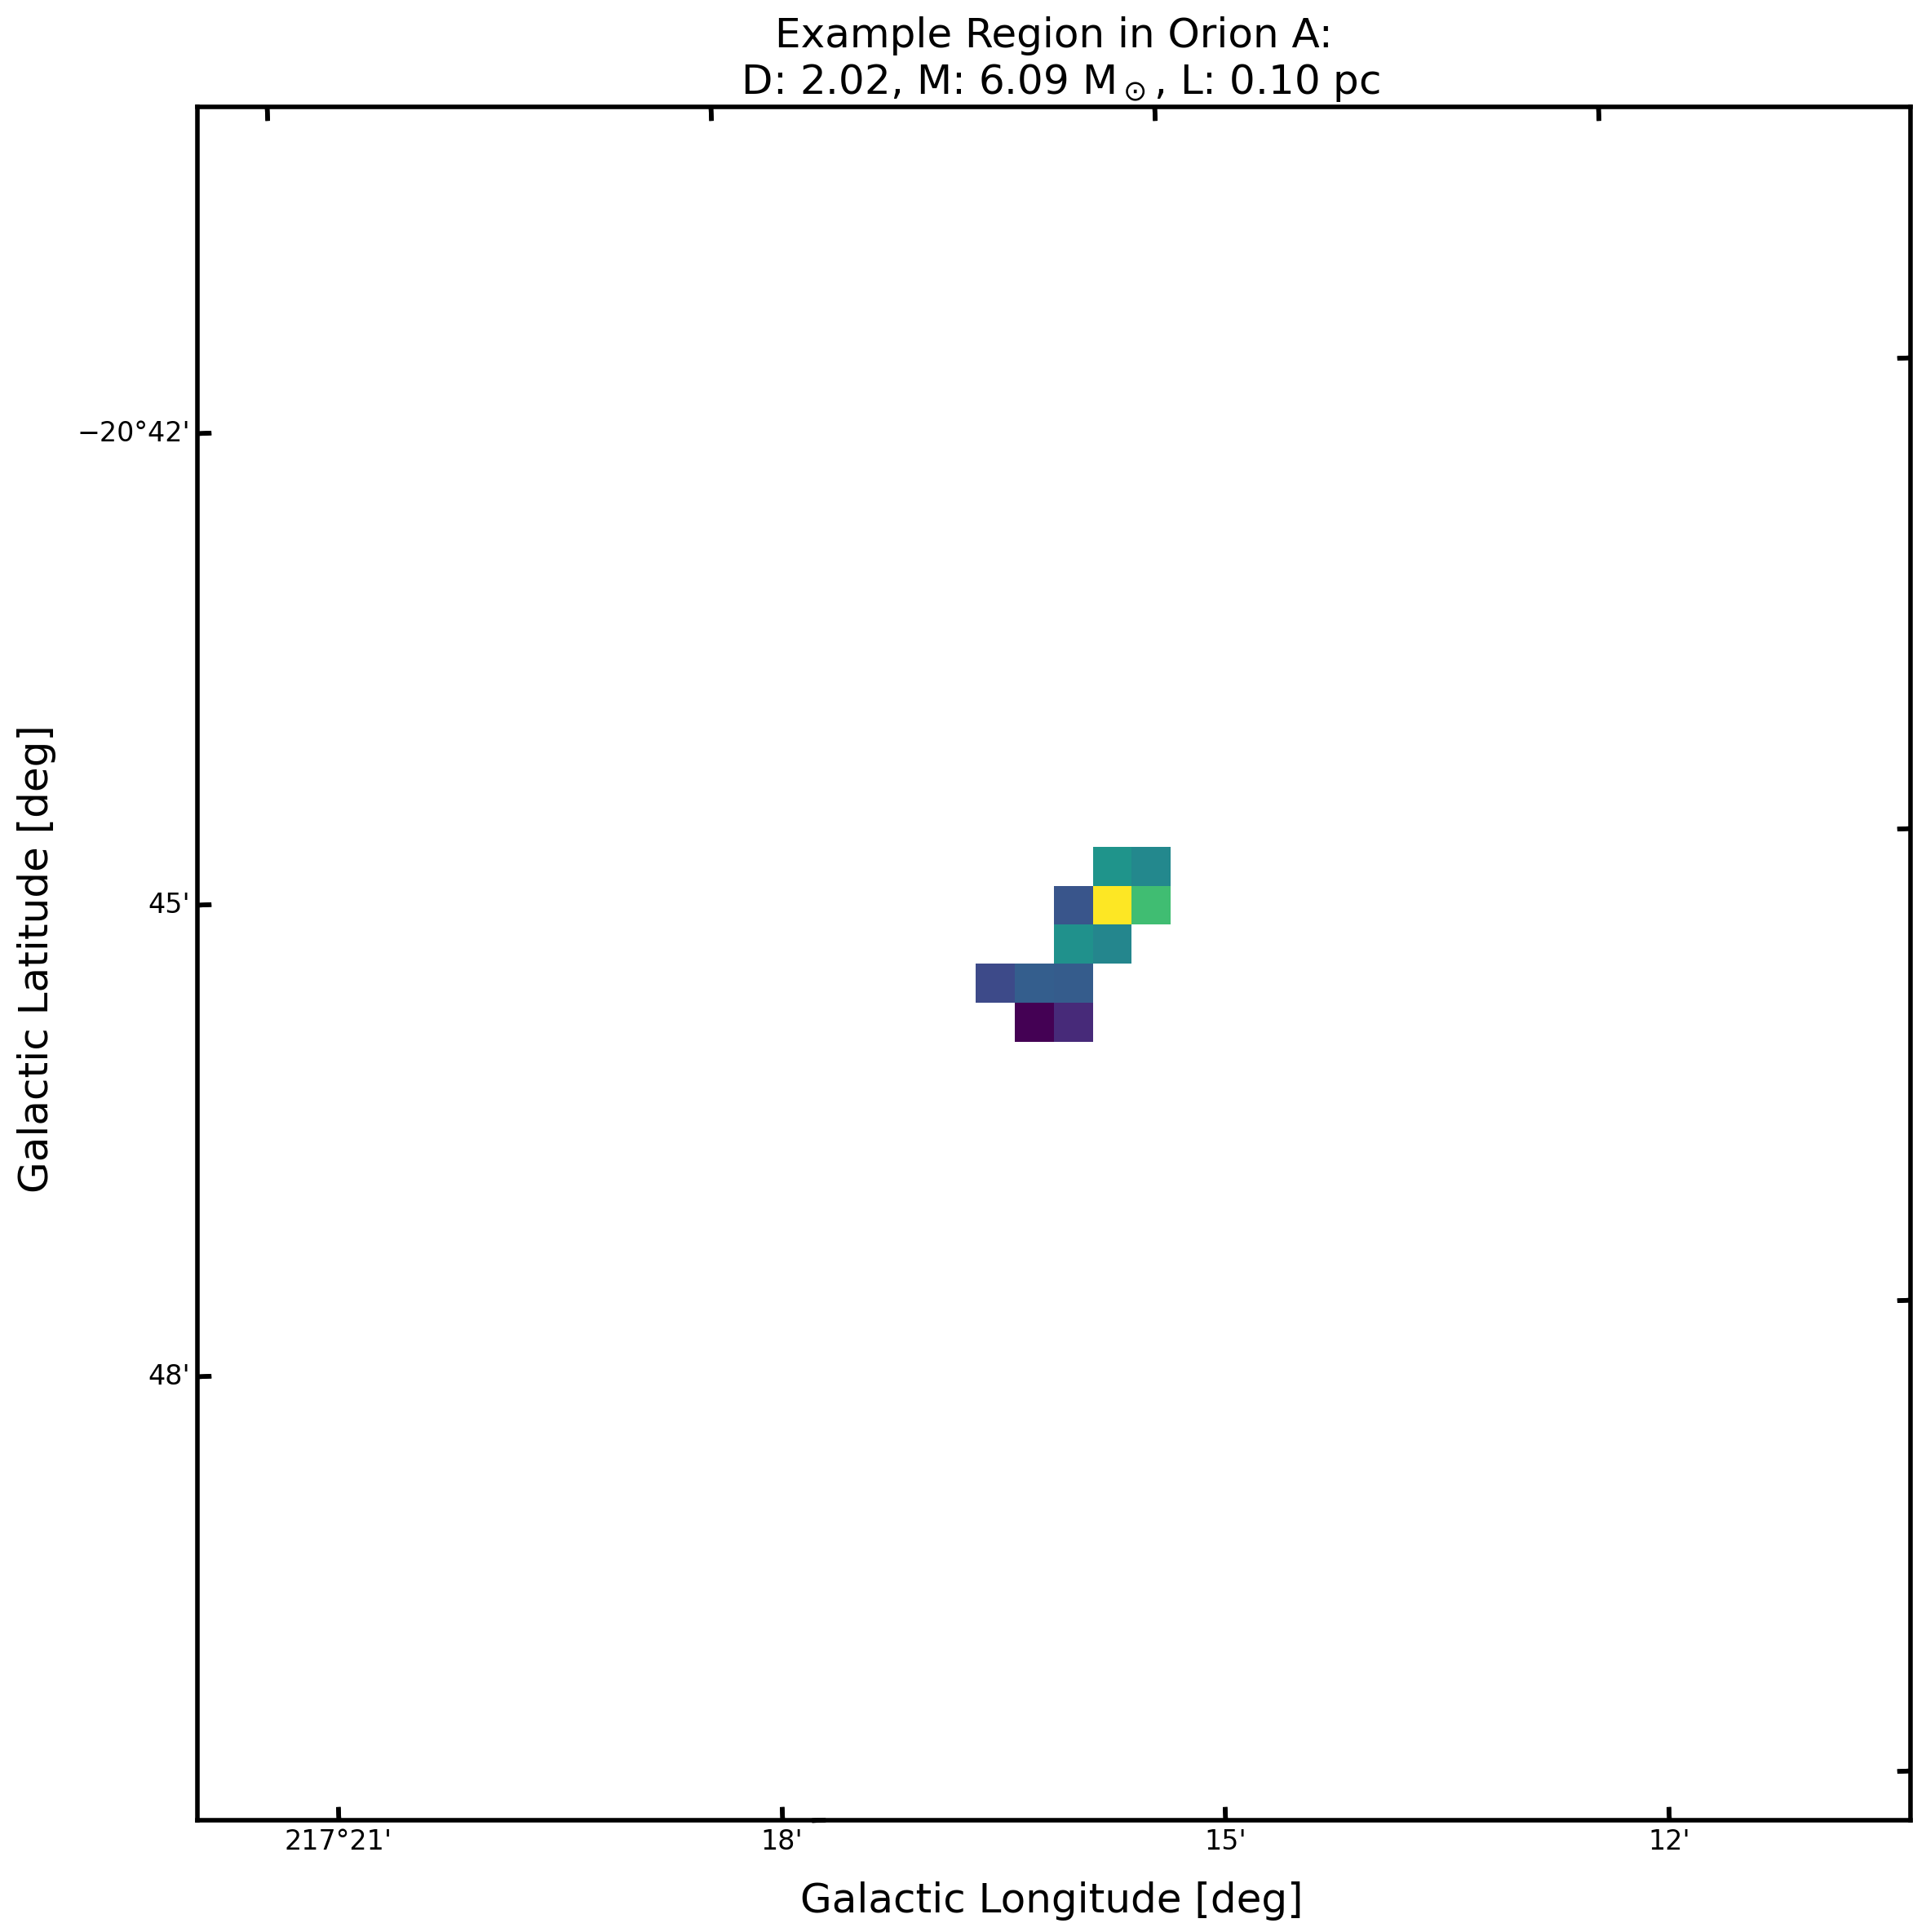
\includegraphics[width=0.6\textwidth]{figures/MSD_Gallery_Orion_A_5.png}
    \caption{Example of the mask of an individual structure extracted from Orion~A at a given column density threshold.}
    \label{fig:gallery_MSD_A_5}
\end{figure}

\newpage

\begin{figure}[h]
    \centering
    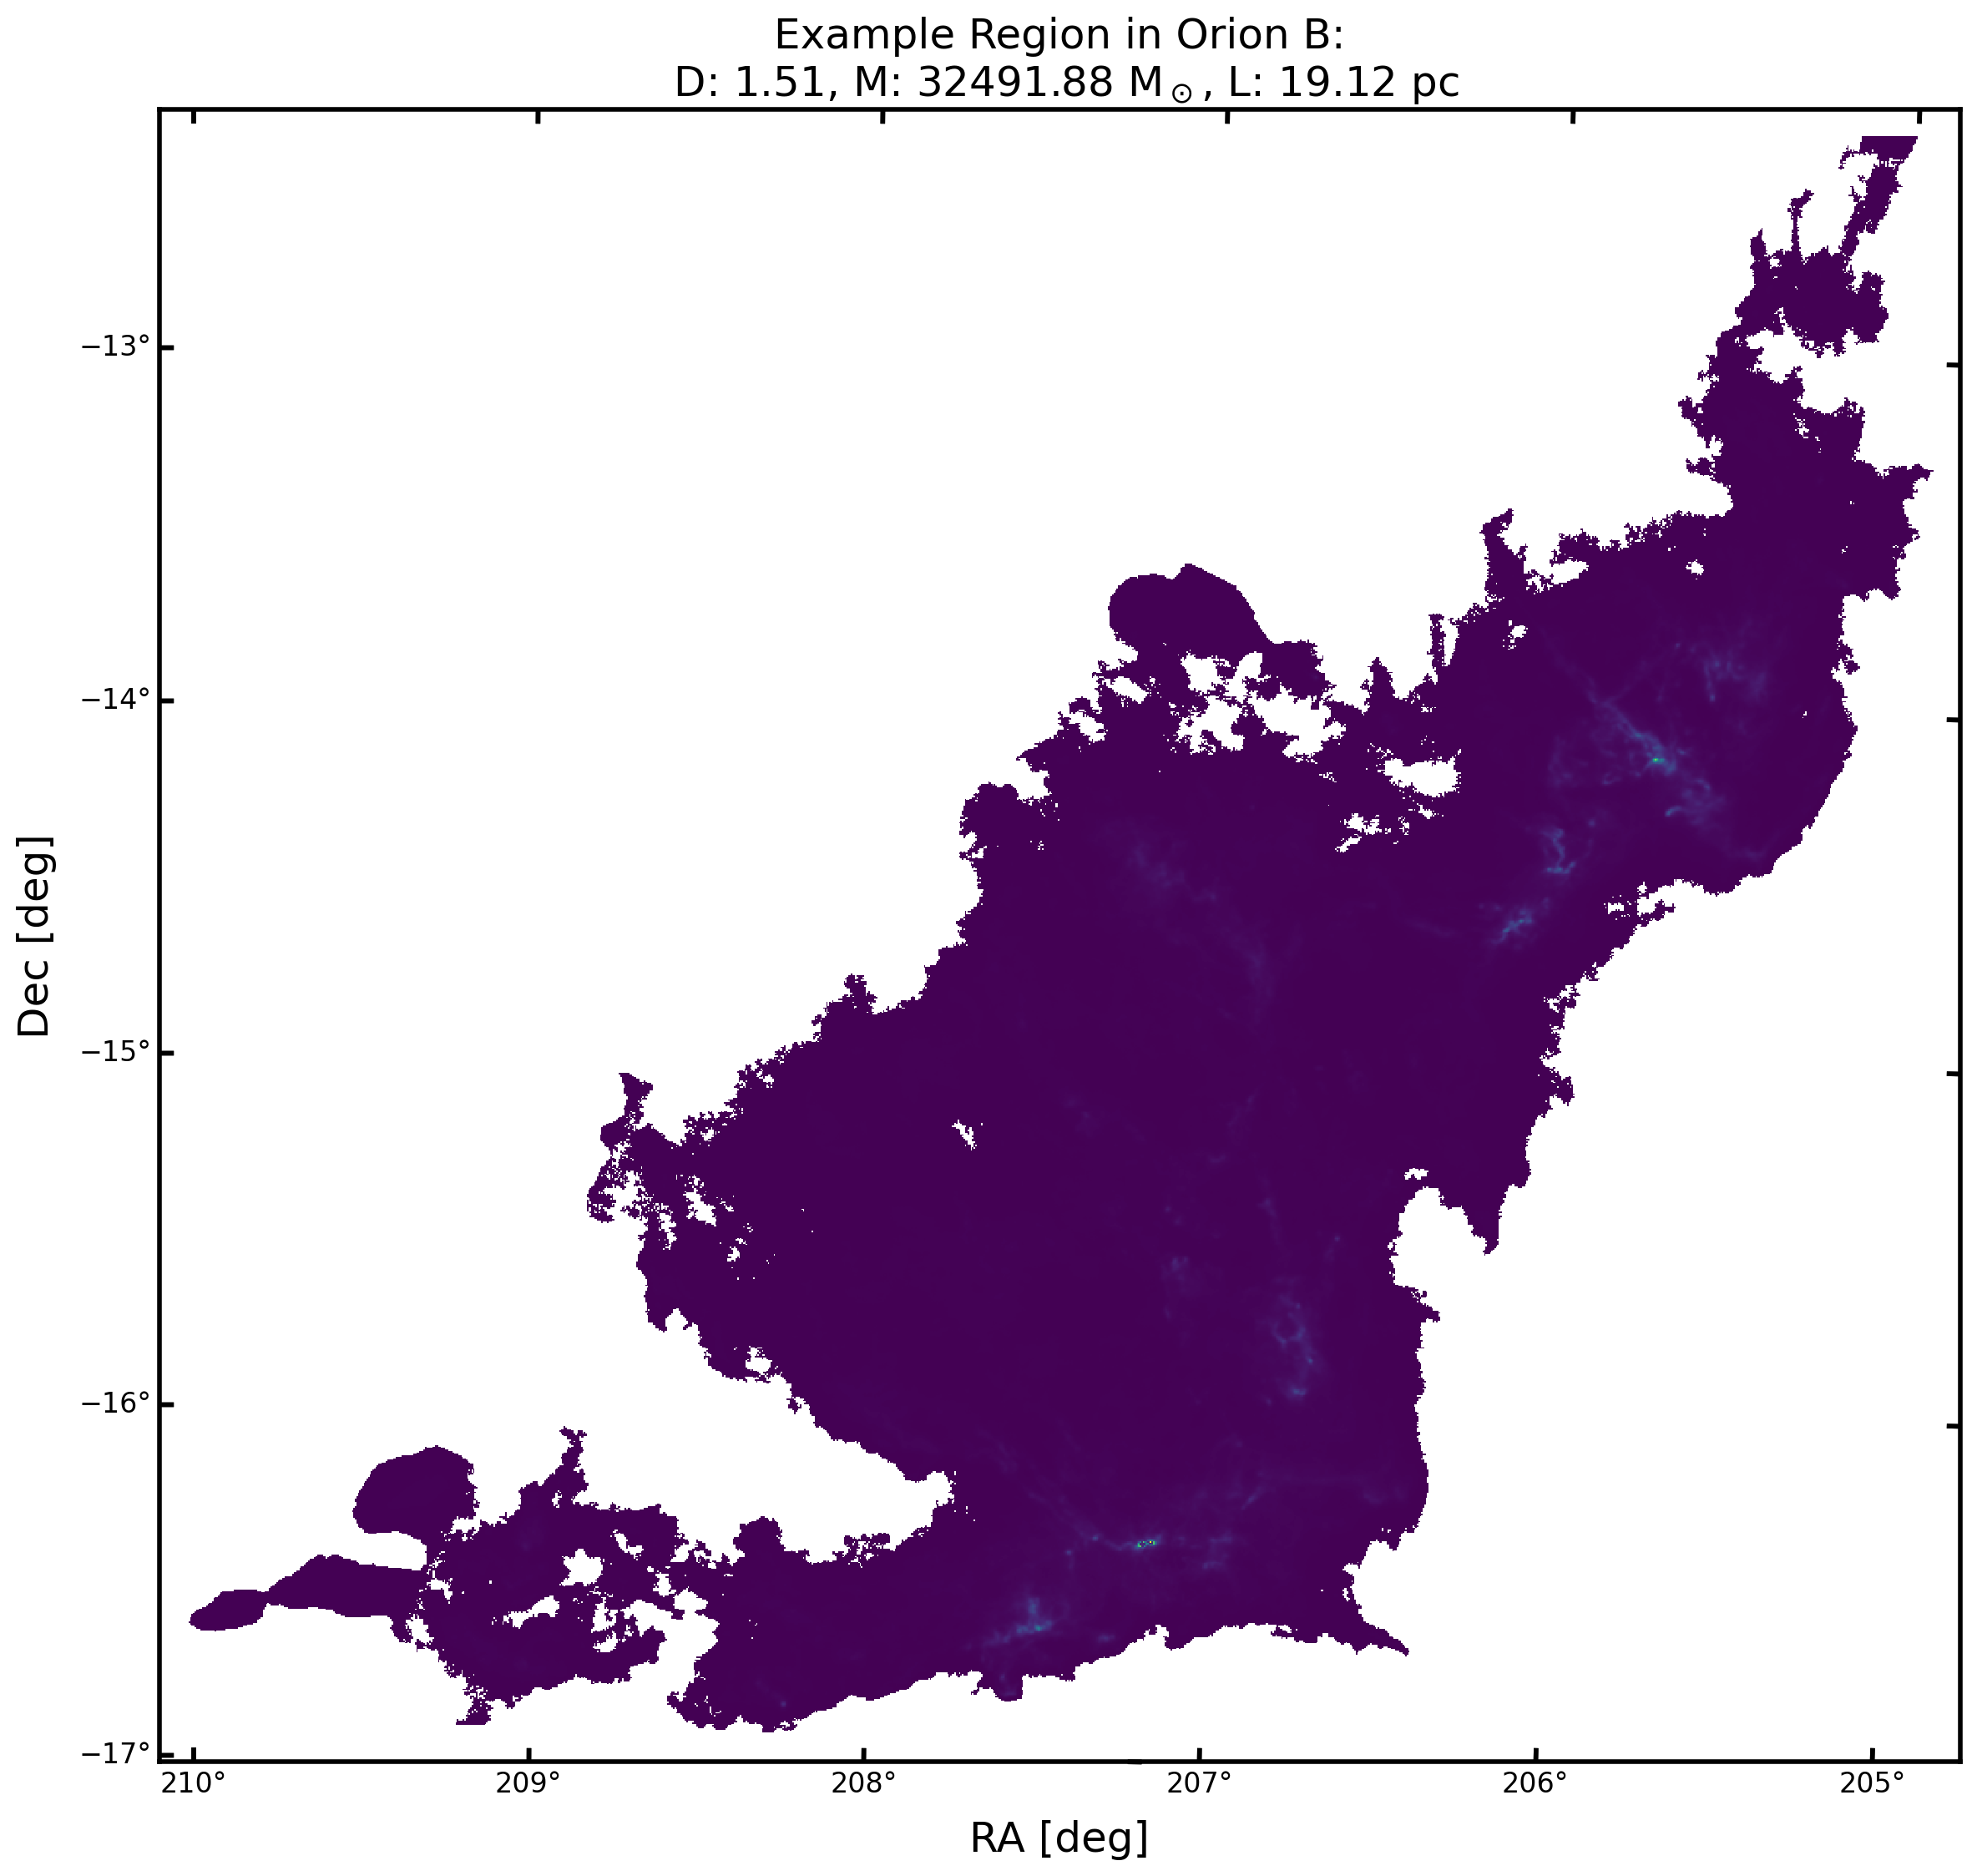
\includegraphics[width=0.64\textwidth]{figures/MSD_Gallery_Orion_B_1.png}
    \caption{Example of the mask of an individual structure extracted from Orion~B at a given column density threshold. Key physical properties—mass, size, and local fractal dimension—are indicated in the title of the plot.}
    \label{fig:gallery_MSD_B_1}
\end{figure}

\begin{figure}[h]
    \centering
    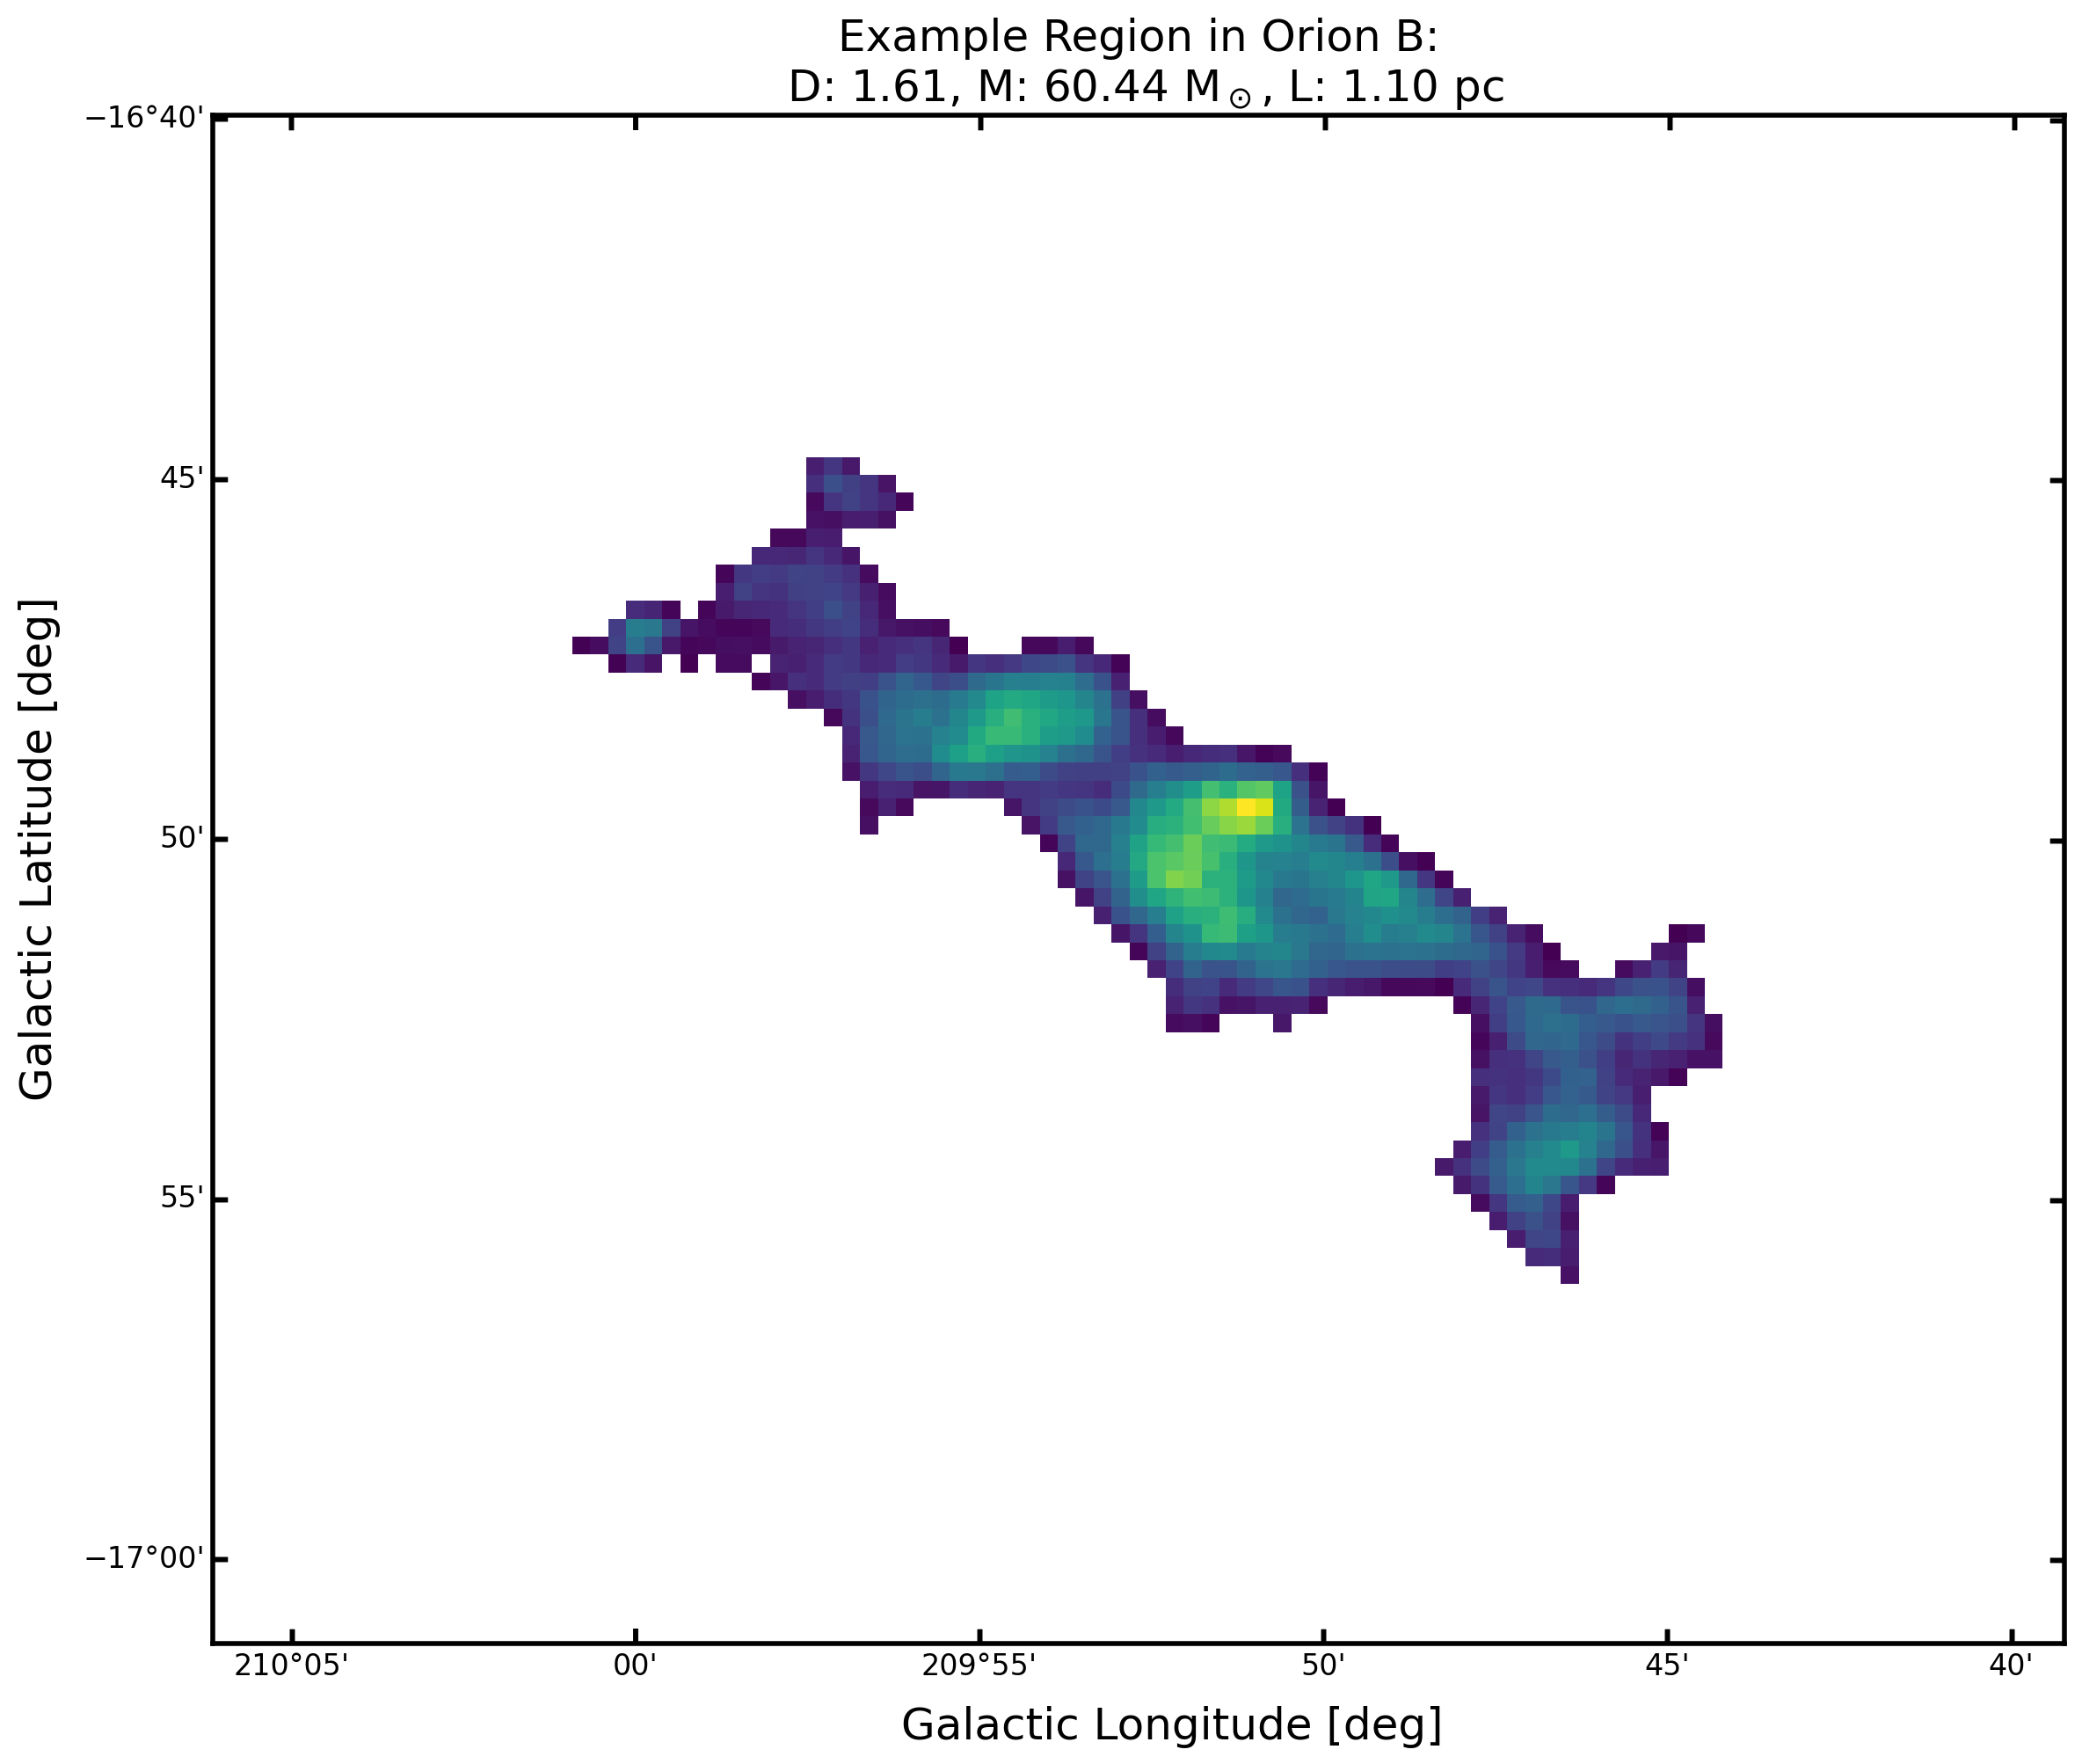
\includegraphics[width=0.64\textwidth]{figures/MSD_Gallery_Orion_B_2.png}
    \caption{Example of the mask of an individual structure extracted from Orion~B at a given column density threshold.}
    \label{fig:gallery_MSD_B_2}
\end{figure}

\begin{figure}[h]
    \centering
    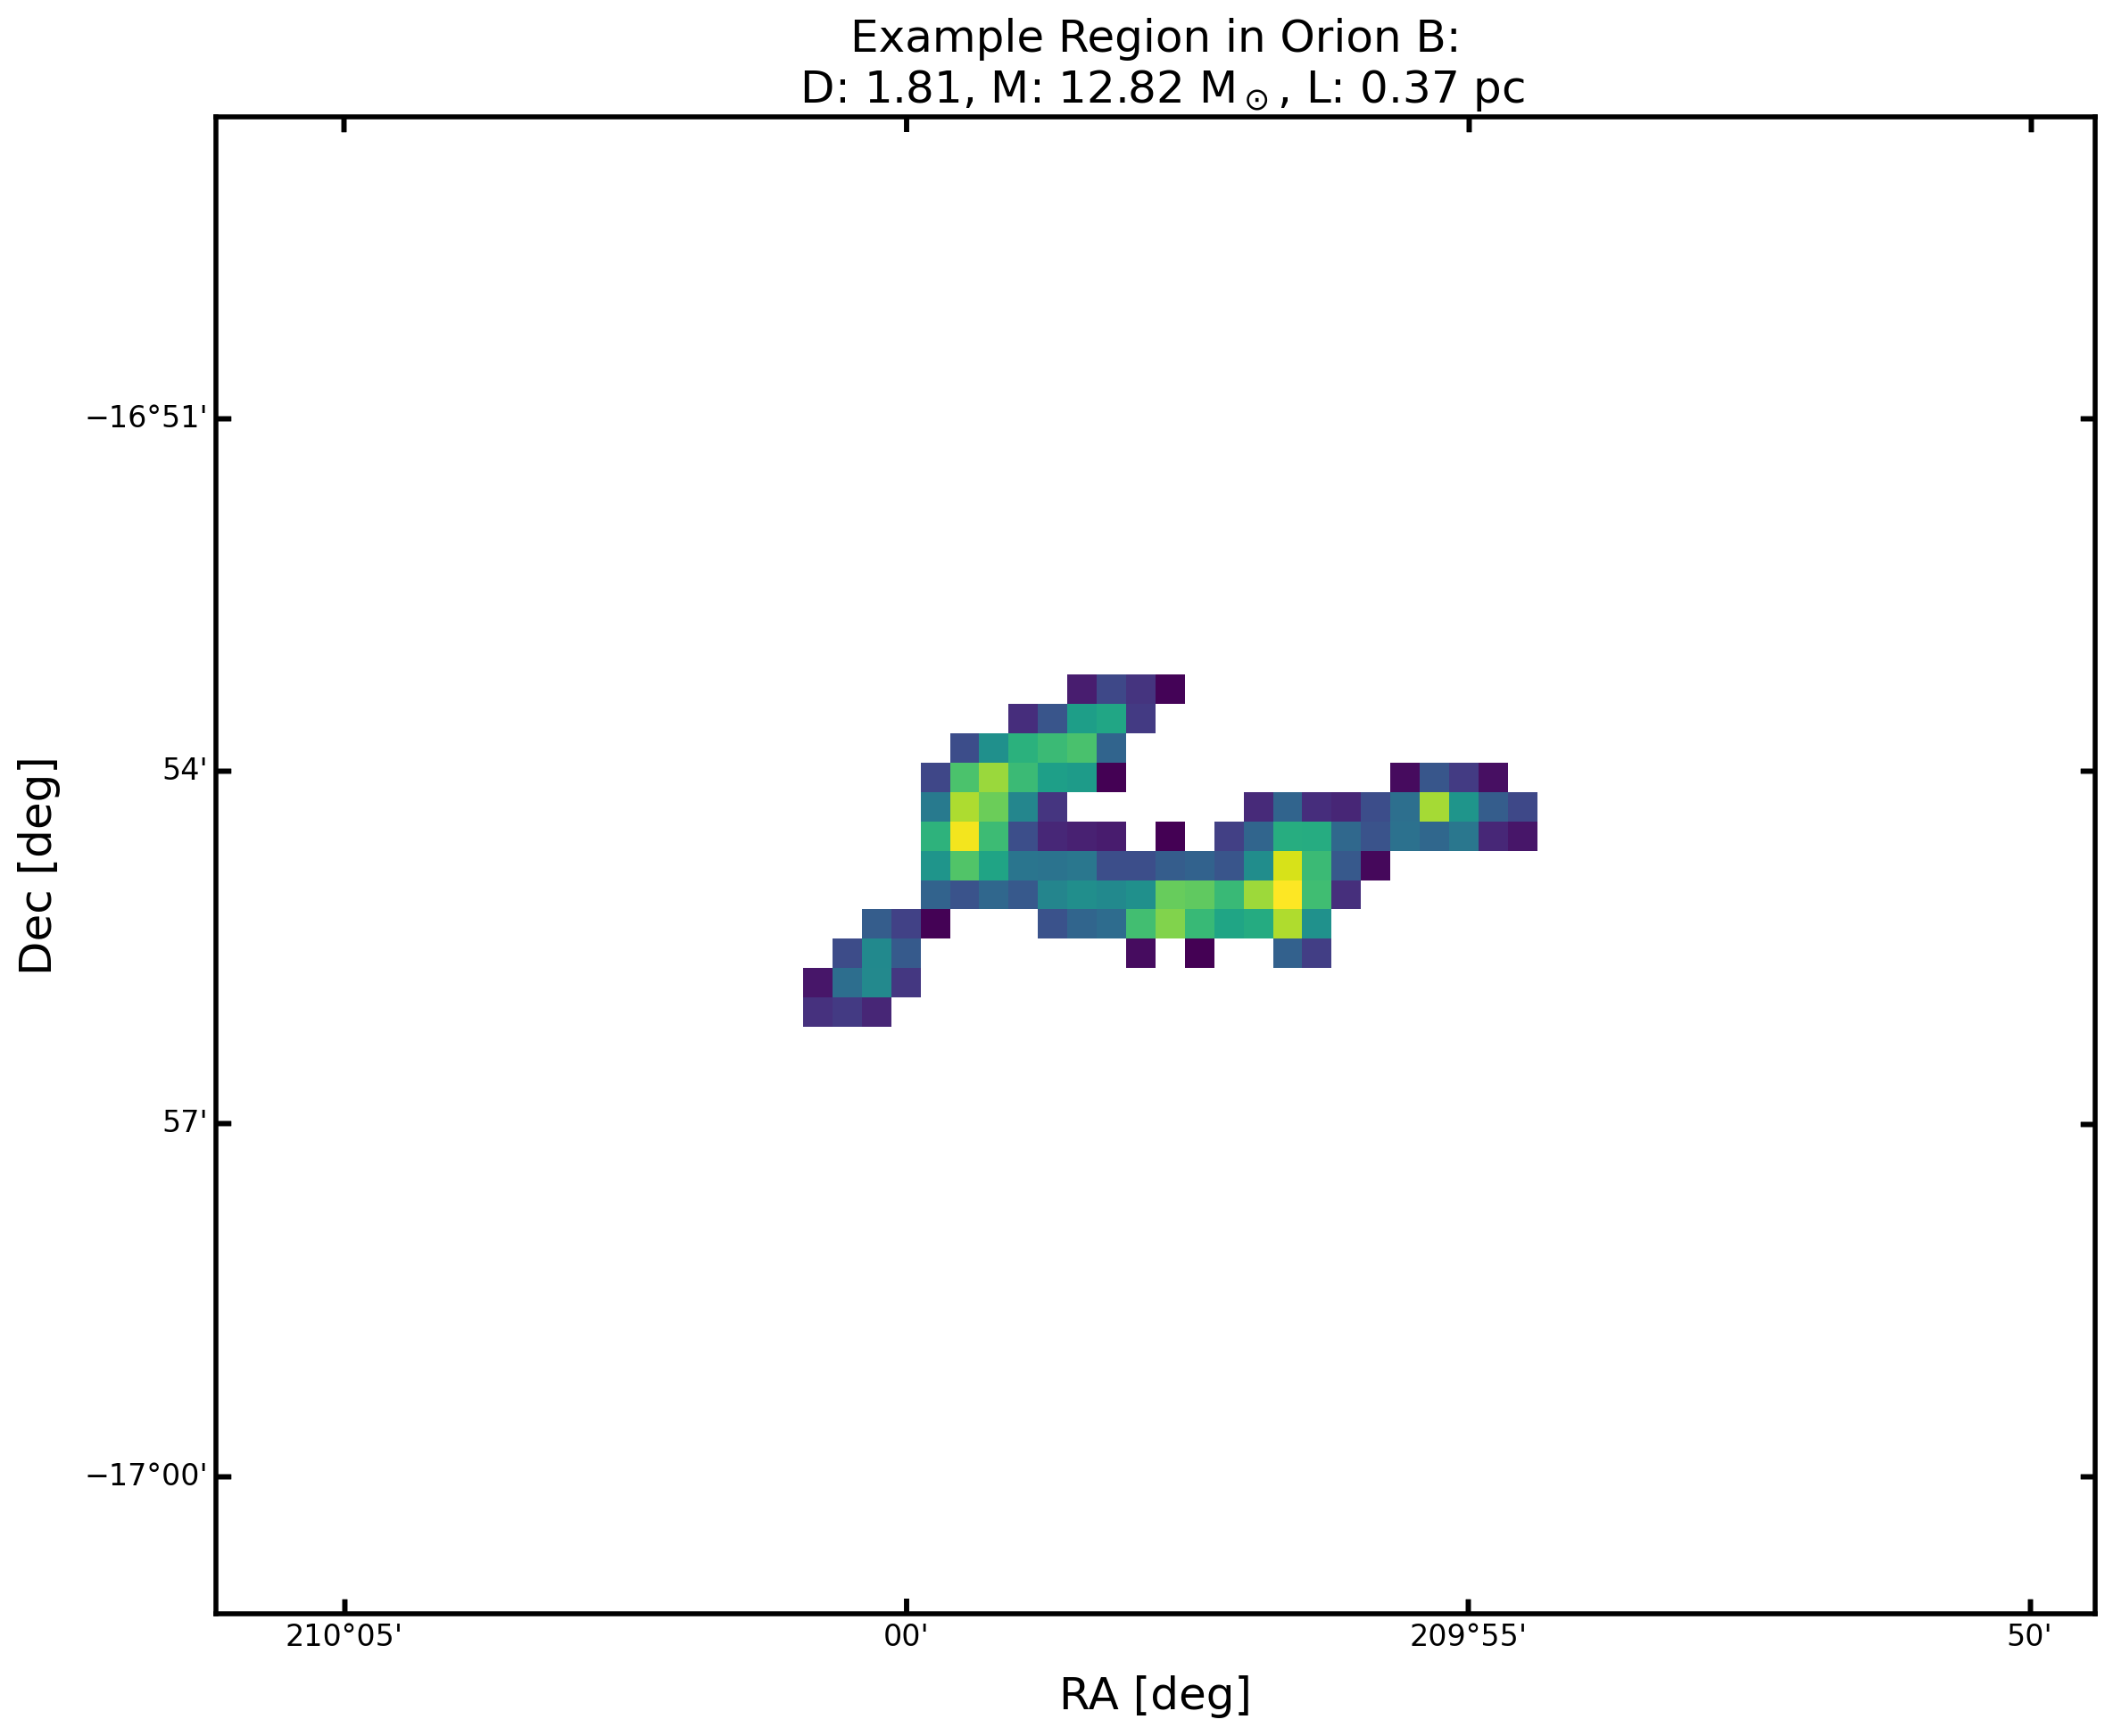
\includegraphics[width=0.64\textwidth]{figures/MSD_Gallery_Orion_B_3.png}
    \caption{Example of the mask of an individual structure extracted from Orion~B at a given column density threshold.}
    \label{fig:gallery_MSD_B_3}
\end{figure}

\begin{figure}[h]
    \centering
    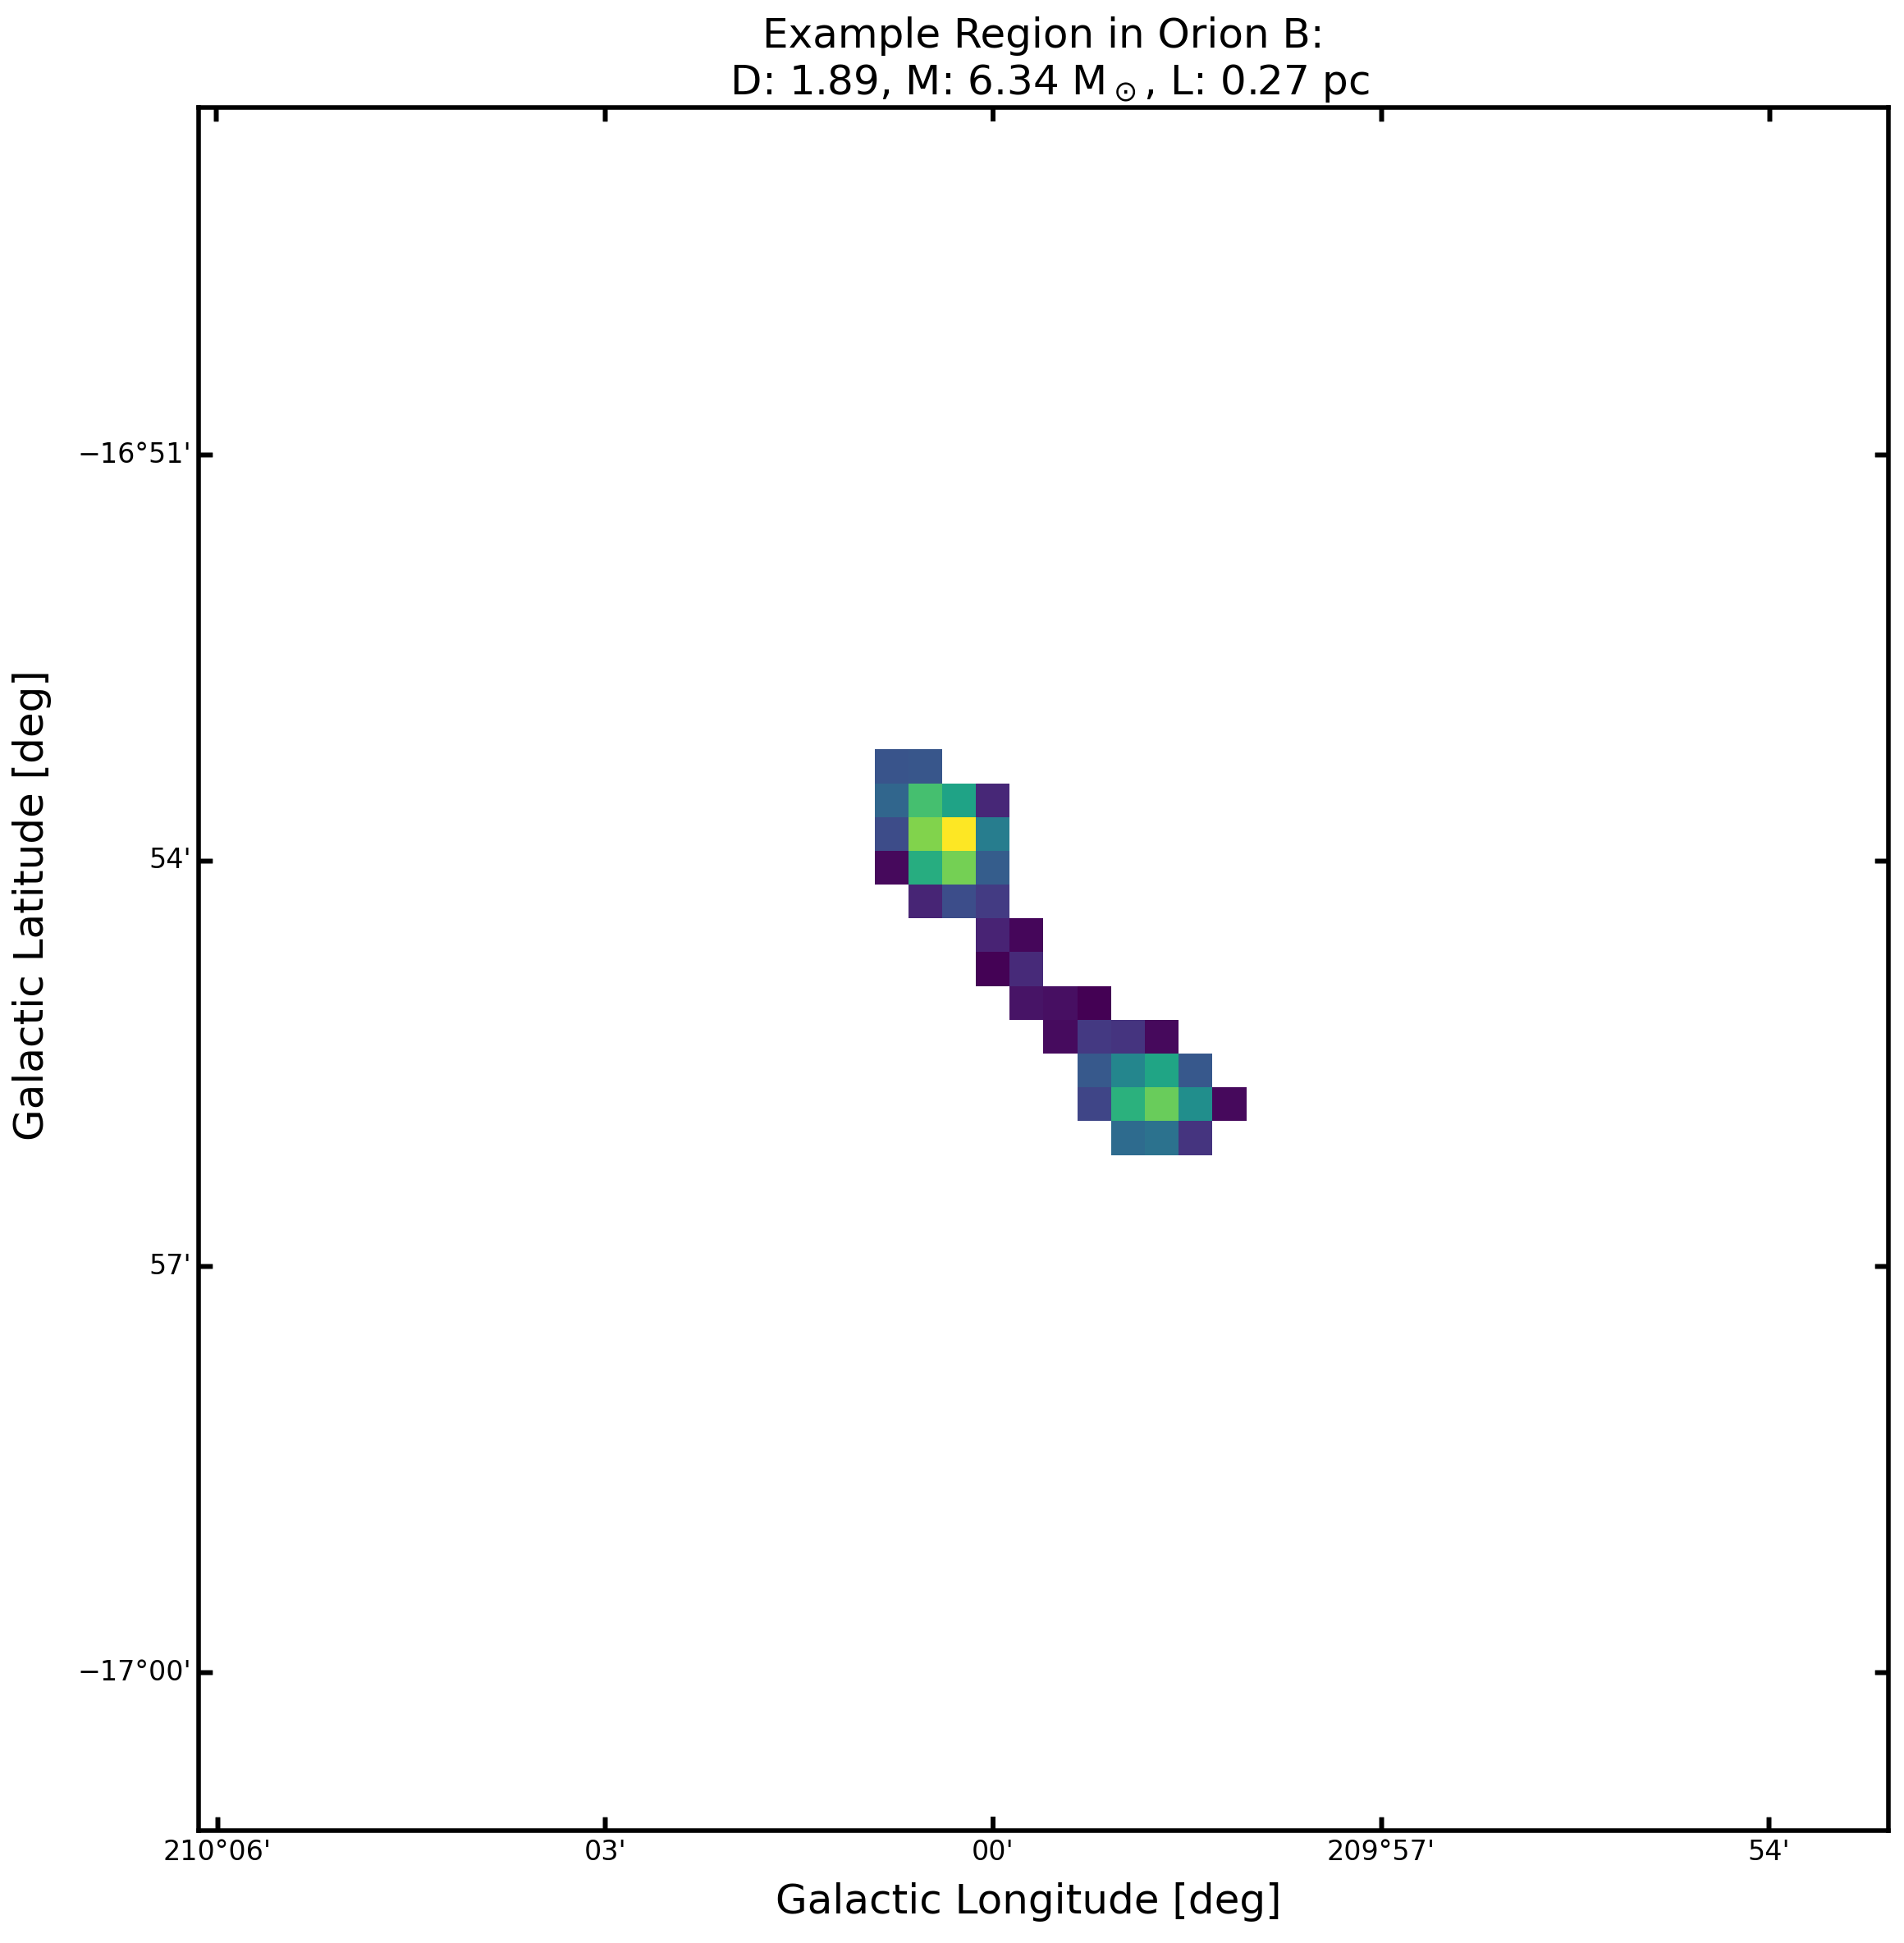
\includegraphics[width=0.64\textwidth]{figures/MSD_Gallery_Orion_B_4.png}
    \caption{Example of the mask of an individual structure extracted from Orion~B at a given column density threshold.}
    \label{fig:gallery_MSD_B_4}
\end{figure}

\begin{figure}[h]
    \centering
    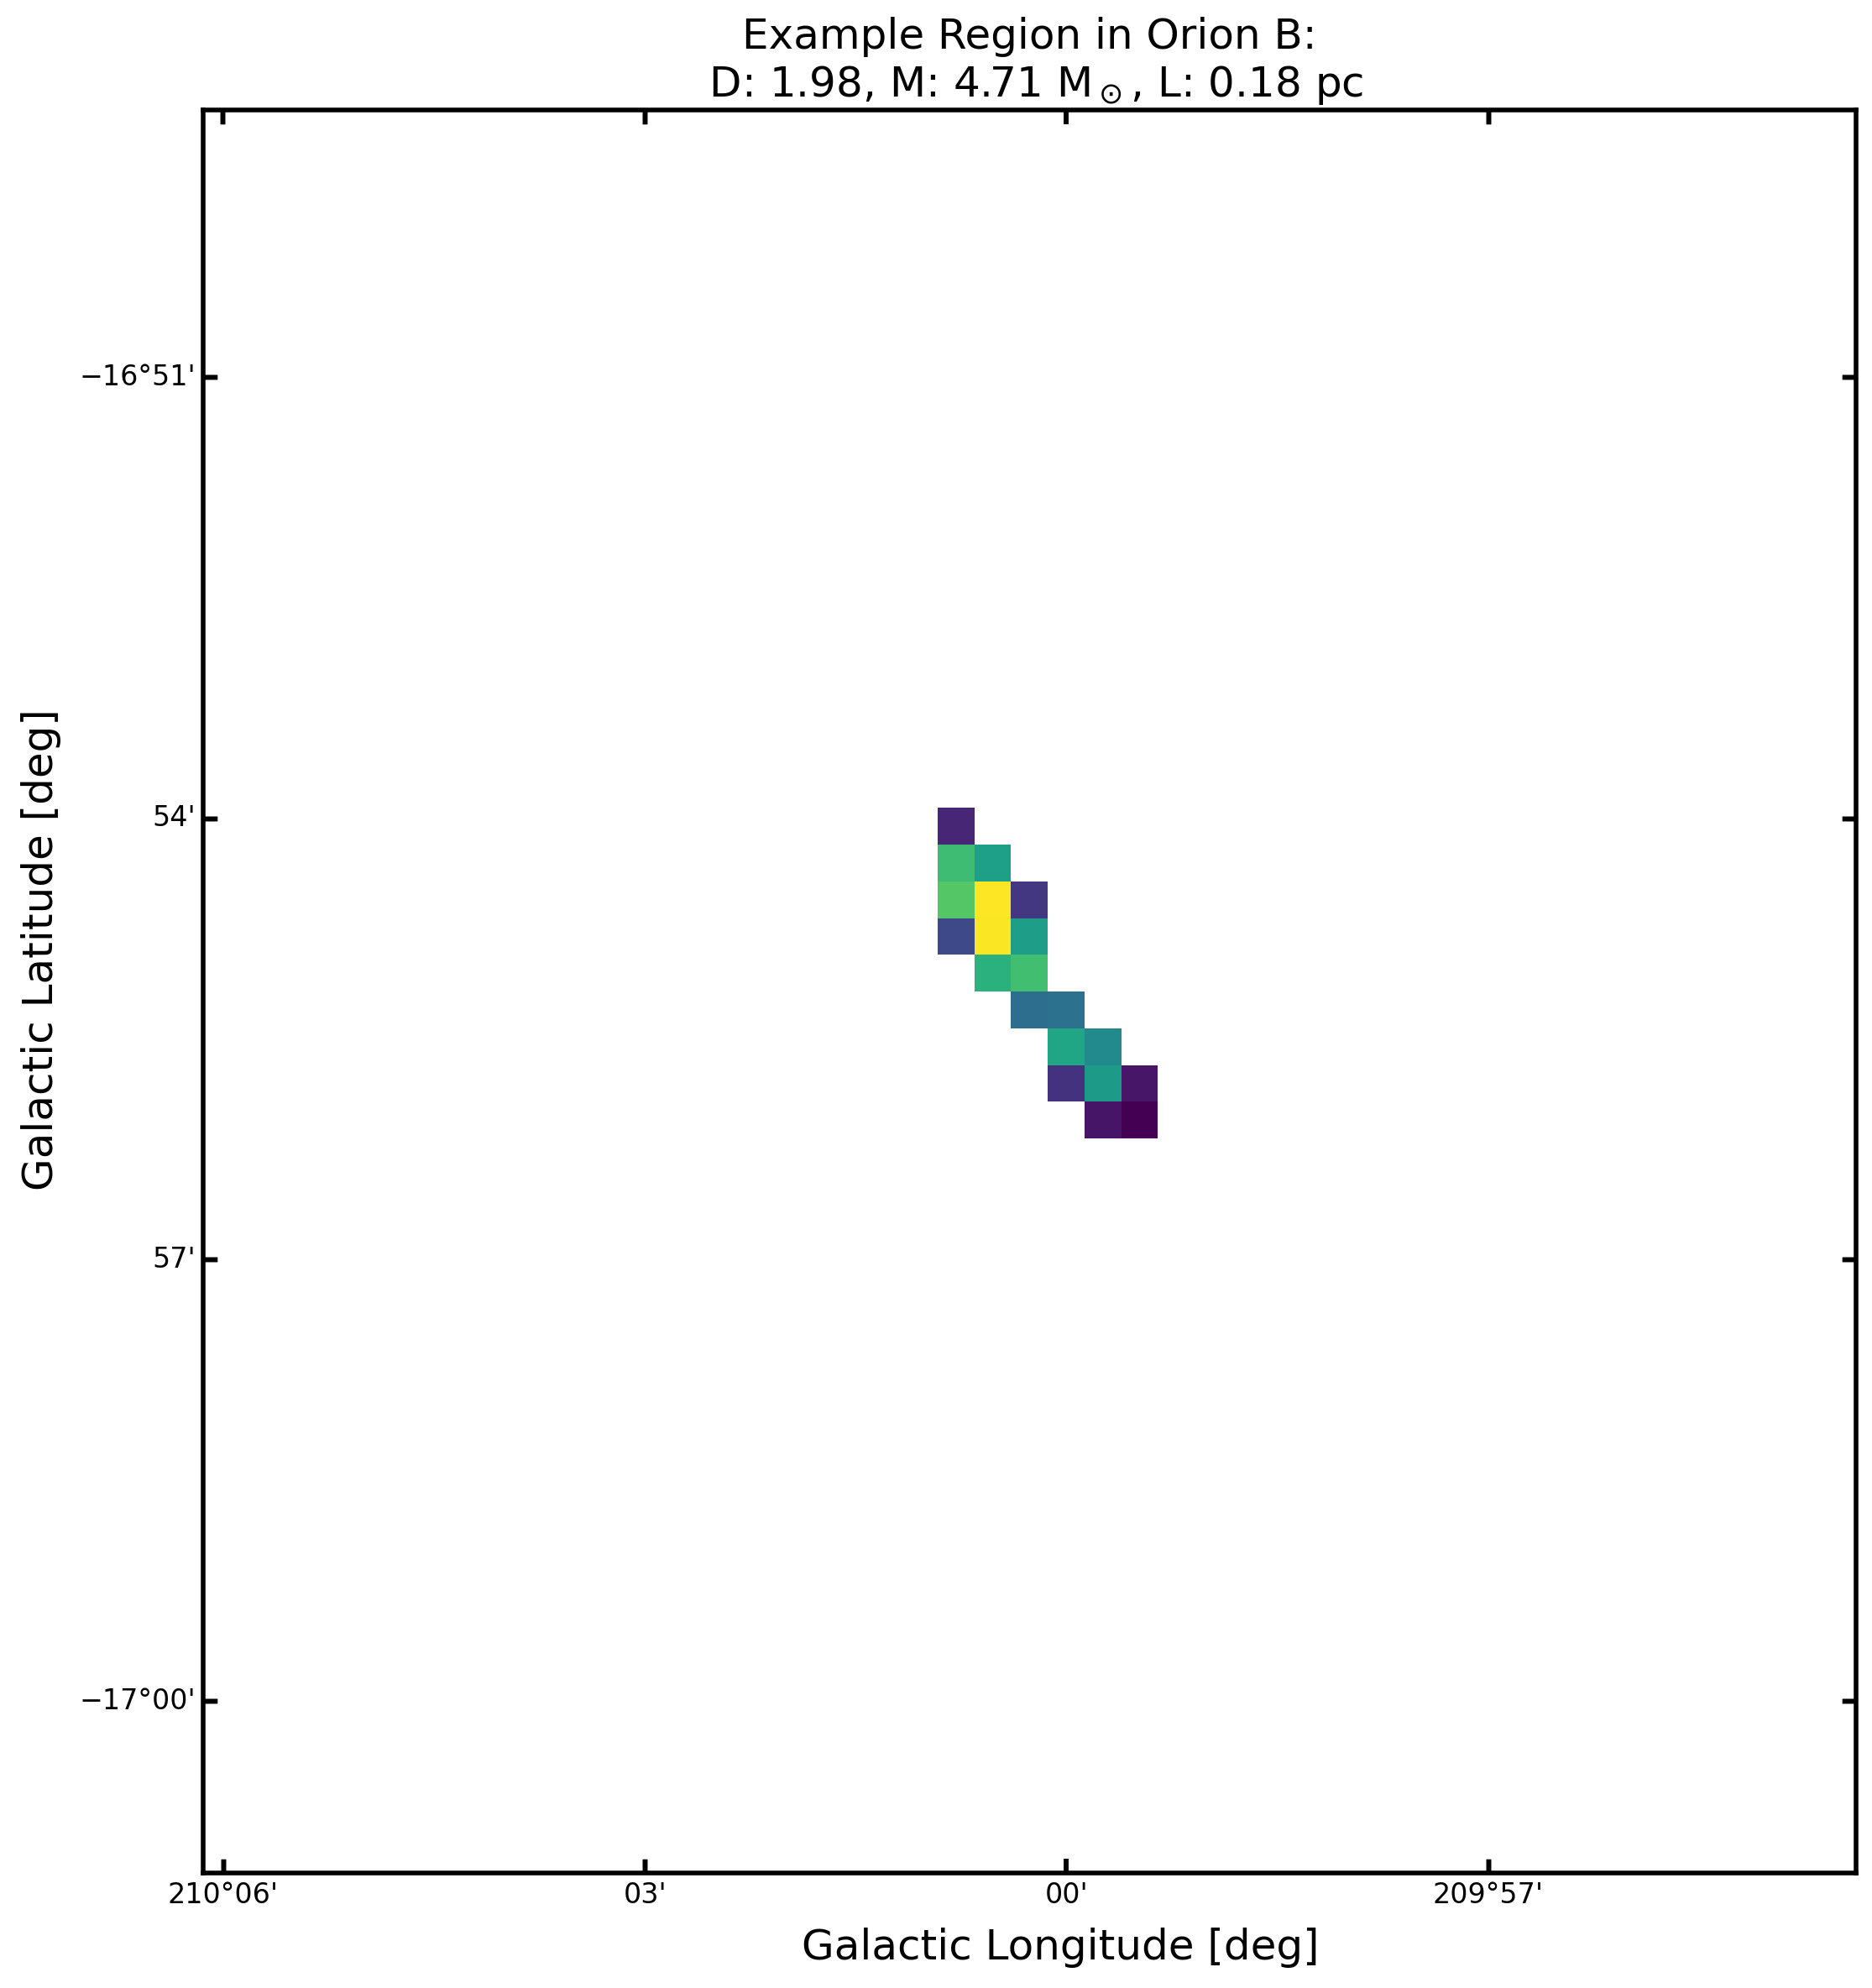
\includegraphics[width=0.64\textwidth]{figures/MSD_Gallery_Orion_B_5.png}
    \caption{Example of the mask of an individual structure extracted from Orion~B at a given column density threshold.}
    \label{fig:gallery_MSD_B_5}
\end{figure}

